\documentclass[11pt]{article}
%\documentclass[11pt,dvipdfm]{article} 

\usepackage{deauthor,times,graphicx}
%\usepackage[hidelinks]{hyperref}
\usepackage{tcolorbox}
%\graphicspath{{istvan/}} 
\usepackage{xpatch}
\usepackage{xspace}
\usepackage{multirow}


\makeatletter

\makeatletter

\newcommand{\hi}[1]{\noindent {\bf #1}}

\newcommand{\lgl}[1]{{\textcolor{blue}{{#1}}}}

\newcommand{\oursys}{\textsf{XuanYuan}\xspace}

\begin{document}

%\pagestyle{plain}
%\pagenumbering{arabic}


\setcounter{figure}{0}  

% ****************** AUTHORS **************************************

\title{\oursys: An AI-Native Database}

%\author{Zsolt Istv\'{a}n\\ \small IMDEA Software Institute, Madrid, Spain\\  \small \{first.lastname@imdea.org\}}
\author{Guoliang Li, Xuanhe Zhou, Sihao Li\\ 
\small Department of Computer Science,Tsinghua University, Beijing, China\\
\small Gauss Database Group, Huawei Company\\  
\small liguoliang@tsinghua.edu.cn}

\maketitle

\begin{abstract}
Online job platforms have proliferated in the last few years.
We anticipate a future where there exists thousands of such platforms covering wide swathes of tasks.
These include crowdsourcing platforms such as Amazon Mechanical Turk (AMT), CrowdWorks, Figure Eight;
specialized services such as ride-hailing;
matching markets such as TaskRabbit that matches workers with local demand and so on.
It is widely anticipated that a vast majority of human workforce will be employed in these platforms.
In this article, we initiate discussions about the under studied aspect of \emph{platform design} --
how to design platforms that maximize the satisfaction of various stakeholders.
We also contribute a novel taxonomy for platform ecosystems
that categorizes existing and emerging platforms.
Finally, we discuss the need for interoperability between these platforms
so that workers and requesters are not tied to a single platform.
\end{abstract}

%!TEX root = ../main.tex

\section{INTRODUCTION}
\label{sec: introduction}


Databases have played a very important role in many applications and been widely deployed in many fields. Over the past fifty years, databases have undergone three main revolutions. 
% what how where example

The first generation is stand-alone databases, which address the problems of data storage, data management and query processing~\cite{DBLP:books/daglib/0006734}. The representative systems include PostgreSQL and MySQL. 
	
	%It centralizes data management under the supervision of the data experts and provides uniform interface to data. 
	%And it is mainly for single-machine applications. 
	%Examples include Postgre95 and the early IBM relational database systems. 

The second generation is cluster databases, which aim to provide high availability and reliability for critical business applications. The representative systems include Oracle RAC, DB2 and SQL server. 
 
	%Database clustering technique is to use multiple machines together to store the same data (data redundancy). 
	%It is mainly applied in fault tolerant environments.
%	Examples include Oracle RAC, MongoDB Replication, Master Slave Replication in MySQL and etc.

The third generation is distributed databases (and cloud-native databases), which aim to address the problems of elastic computing and dynamic data migration in the era of big data~\cite{DBLP:journals/jidm/FigueiredoBM10}. The representative systems include Aurora~\footnote{https://aws.amazon.com/cn/rds/aurora/} and GaussDB~\footnote{https://e.huawei.com/en/solutions/cloud-computing/big-data/gaussdb-distributed-database}. 
	
%	Firstly, with distributed processing, it can further distribute the workload among working nodes~\cite{DBLP:journals/jidm/FigueiredoBM10}. Secondly, with Database as a Service (DBaaS), cloud database allows companies to free up personnel and focus on important tasks. Besides, cloud database makes it easy to scale up or down their databases with virtual technology. 
%	It is mainly applied for data-intensive applications.
%	Examples include GCP, AWS RDS, Microsoft Azure and etc.

% big data era, database systems face three challenges. Firstly, the traditional empirical optimization techniques (e.g., cost estimation, join order selection, knob tuning) cannot meet the high-performance requirement for large-scale data, various applications and diversified users. We aim to  design learning-based techniques to make database more intelligent. Secondly, many database applications require to use AI algorithms, e.g., image search in database. We can embed AI algorithms into database, utilize database techniques to accelerate AI algorithms, and provide AI capability inside databases. Thirdly, traditional databases focus on using general hardware (e.g., CPU), but cannot fully utilize new hardware (e.g., ARM, AI chips). Moreover, besides relational model, we can utilize tensor model to accelerate AI operations. Thus, we need to design new techniques to make full use of new hardware. 

However, the traditional databases still have several limitations in the big data era, due to the large-scale data, various applications/users and diversified computing power.

(1) Traditional database design is still based on empirical methodologies and specifications, and require heavy human involvement (e.g., DBAs) to tune and maintain the databases. We use several examples to show that databases can be improved using AI techniques. First, databases have hundreds of knobs and it requires DBAs to tune the knobs to adapt to different scenarios. Recently the database committee attempts to utilize machine learning techniques~\cite{DBLP:conf/sigmod/AkenPGZ17, DBLP:conf/vldb/qtune19,  DBLP:conf/sigmod/cdbtune19} to automatically tune the knobs, which can achieve better results than DBAs. Second, database optimizer relies on cost and cardinality estimation but traditional techniques cannot provide accurate estimation. Recently deep learning based techniques~\cite{DBLP:conf/cidr/KipfKRLBK19, DBLP:conf/sigmod/OrtizBGK18} are proposed to estimate the cost and cardinality which also achieve better results. Moreover, learning-based optimizers~\cite{DBLP:journals/corr/abs-1808-03196, DBLP:conf/sigmod/MarcusP18}, learning-based  index recommendation~\cite{DBLP:conf/hais/PedrozoNR18}, learning-based automatic view generation~\cite{DBLP:journals/corr/abs-1903-01363} provide alternative optimization opportunities for database design. Third, traditional databases are designed by database  architects based on their experiences. Recently some learning-based self-designed techniques are proposed, e.g., learned indexes~\cite{DBLP:conf/sigmod/KraskaBCDP18} and learned NoSQL database design~\cite{DBLP:conf/cidr/IdreosDQAHRLJGL19}. Thus we can utilize AI techniques to enhance databases and make databases more intelligent.      


%They are not intelligent. Databases are unaware of workload type and try to use one mode to fit all. For example, the database parameters are static and need to be adjusted manually for different scenarios. 


(2) Traditional databases focus on {\it relational model} and provide relational data management and analysis ability. However, in the big data era, there are more and more diverse data (e.g., graph data, time-series data, spatial data, array data) and applications (e.g., machine learning and graph computing). It calls for a new database system that can integrate multiple models (e.g., relational model, graph model, tensor model) to support diversified applications (e.g., relational data analysis, graph computing and machine learning). Moreover, we can embed AI algorithms into databases, design in-database machine learning frameworks, utilize database techniques to accelerate AI algorithms, and provide AI capability inside databases.

%They are not integrated. Databases are usually based on single data model and cannot support integrated data analysis (IDA). Because now most databases store data in well-defined schemas (static) and only support structured data analysis.  It's expensive to aggregate data from different databases.
%emails, text files, web pages, digital images, multimedia content, navigation details and social media posts.

(3) Transitional databases only consider general-purpose hardware, e.g., CPU, RAM and disk, but cannot make full use of new hardware, e.g., ARM, AI chips, GPU, FPGA, NVM, RDMA. It calls for a heterogeneous computing framework that can efficiently utilize diversified computing powers to support data management, data analysis, and in-database machine learning. 

% operations.


% AI-Naive: idea contributions		
To address these problems, we propose an AI-native database (\oursys), which not only integrates AI techniques into database to make database more intelligent but also provides in-database AI capabilities. In particular, on one hand, \oursys integrates AI techniques into databases to provide self-configuring, self-optimizing, self-monitoring, self-diagnosis, self-healing, self-security and self-assembling capabilities for databases, which can improve the database's availability, performance and stability, and reduce the burden of intensive human involvement. On the other hand, \oursys enables databases to provide AI capabilities using declarative languages, in order to lower the barrier of using AI. Moreover, \oursys also fully utilizes diversified computing power to support data analysis and machine learning. 

An AI-native database can be divided into five stages. The first is AI-advised database, which takes an AI engine as a plug-in service and provides offline database suggestions, e.g., offline index advisor, offline knob tuning. The second stage is AI-assisted database, which takes an AI engine as a built-in service and provides online monitoring and suggestions, e.g., online statistics collection, online database state monitoring, and online diagnosis. The third is AI-enhanced database. One one hand, it provides AI based database components, e.g., learned index, learned optimizer, learned cost estimation, learned storage layout. On the other hand, it provides in-database AI algorithms and accelerators. The fourth is AI-assembled database, which provides multiple data models (e.g., relational model, graph model, tensor model) and fully utilizes the new hardware to support heterogeneous computing. It can provide multiple options for each component, e.g., learned optimizer, cost-based optimizer, and rule-based optimizer, and thus can automatically assemble the components to form a database in order to achieve the best performance for different scenarios. This is similar to AlphaGO, which can explore more optimization spaces than humans. The fifth is AI-designed database, which integrates AI into the life cycle of database design, development,  evaluation, and maintenance, which provides the best performance for every scenario. 


In this paper, we first present the details of AI-native databases and then provide the research challenges and opportunities for designing an AI-native database. 

%outside database and provide we pack AI tools into the database to achieve auxiliary optimization. Second, we implant them into the DB kernel to improve efficiency. Third, we reshape DB kernel based on AI tech and provide unified engine to provide both DB and AI services. Fourth, we deploy heterogeneous computing architecture to better support operations of both DB and AI. Finally, we 


%We make the following contributions in this paper.

%\noindent (1) 

%We propose a practical way to achieve AI-native database in five stages (see Section~\ref{sec:work}).   

%\noindent (2) We propose an AI-advised database, which packs AI tools to provides auxiliary optimization (see Section~\ref{subsec: advised}). 

%\noindent (3) We propose an AI-Assisted database, which implants AI tools into DB kernel to provide runtime optimization (see Section~\ref{subsec: assisted}).

%\noindent (4) We propose an AI-Enhanced database, which incorporates AI tech into DB kernel and provides unified engine to provide DB and AI services (see Section~\ref{subsec: enhanced}).

%\noindent (5) We propose an AI-Assembled database, which provides heterogeneous computing architecture to enhance DB and AI services (see Section~\ref{subsec: assemble}).

%\noindent (6) We propose an AI-Designed database, which integrates AI theory into its life cycle to achieve a real AI-native database (see Section~\ref{subsec: designed}).



%
\section{Background on Privacy-Sensitive Mobile Contact Tracing}

The key building block for Privacy-Sensitive Mobile Contact Tracing (PS-MCT) is a subtle combination of radio protocols, cryptography, and risk-calculation.  
Phones have a short-range radio, Bluetooth, used to connect to nearby devices.  
To make those connections it periodically broadcasts tiny bits of information. 
The PS-MCT protocols leverages this short-range background broadcast to resolve nearby individuals.\shankari{Is this the final term we decided on? I recall some pushback from David on the term, and I don't remember this as one of the options. Since our current focus is on the idea and not on a working system, it seems like it is a good idea to get the terminology right}


In the Apple-Google Exposure Notification (AGEN) protocol, each phone generates a daily secret key called a Temporary Exposure Key (TEK).
Then every 15 minutes the phone uses the TEK to generate a new 16 byte Rolling Proximity Identifier (RPI). The RPI sequence is generated using a cryptographic hash function, so it does not carry any information about the source individual.  
The current RPI is then continuously broadcast every few hundred milliseconds.
All phones log the RPIs they hear for future exposure analysis.  
Because the RPI is continuously changing, it also cannot be easily tracked.


When someone tests positive they can \textbf{anonymously} publish the daily keys (TEKs) from the days when they were contagious.  
The confirmed positive collection of TEKs is called a Diagnosis Key in the AGEN protocol.  
The Diagnois Keys are published by sharing them with a trusted server which publishes the TEKs for download.
Others can obtain these keys and use the same cryptographic hash functions to recreate the sequence of RPIs. This sequence, combined with some region-specific weights, can determine if they encountered any infected individuals.  
This entire process is accomplished within the Android and iOS operating systems. Government sanctioned apps are only responsible for authenticating infected individuals and, with user permission, publishing the keys. 

It is important to note the distinction between policy and mechanism. The AGEN protocol (and the extensions proposed in this paper) provide a mechanism to detect and notify users about exposure risk, but it is up to public health authorities to define what constitutes an exposure. This distinction is explored in more detail in section \ref{sec:commons}.



%\section{Motivation}
\label{sec:motivation}

Crowdsourcing platforms has been extremely well studied by different communities~\cite{doan2011crowdsourcing}.
We believe that they are harbingers of the oncoming shift towards the gig economy
brought upon by online job platforms.
By studying how workers fare in these platforms allows us to extrapolate the findings to Future of Work (FoW).

Crowdsourcing platforms including Amazon Mechanical Turk (AMT) and CrowdWorks have a number of similarities
to online job platforms.
Requestors create various tasks that include information such as description of the work required, compensation provided, requestor details etc.
The requestor can also filter workers based on previous experience.
When a worker logs on, she could see all the available tasks and choose to work on a subset of them.
When the worker submits a task, it could be reviewed by the requestor.
If deemed satisfactory, the worker is paid.
If not, the worker submission is rejected.
The crowdsourcing platform takes a cut from the payment made by requestor to the worker.
This basic model pioneered by AMT has become ubiquitous
in online job platforms as diverse as Uber, TaskRabbit and so on.

A number of studies such as~\cite{brawley2016work} have found that there is a large turnover
among workers in Crowdsourcing platforms.
Often, the barriers for turnover is much less steeper than in a traditional employment setting.
This often causes workers to either completely stop working in a platform such as AMT
or have a partial turnover where they just stop working on tasks from a particular requestor.
It is important to address both types of turnover.
The former could be illustrative of dissatisfaction with the platform
whereas the latter could be due to dissatisfaction with requestors.

We collaborated with CrowdWorks, one of the largest crowdsourcing platforms in Japan.
It provides support for more than 200 types of tasks.
%\red{More details about Crowdworks that could be relevant.}
It is used by more than 25000 companies and close to a million active workers. 
We begin by analyzing the turnover rate of workers in CrowdWorks. 
Figure~\ref{fig:persistenceRate} shows what fraction of workers
persist with the platform over a period of time.
One can see that as much as 75\% of workers drop off within couple of months.
The number of workers who persist for more than 2 years is as little as 5\%.
The success of any crowdsourcing platform hinges on successfully retaining workers.
Hence, identifying the factors causing worker turnover and mitigating them is of paramount interest.
It is expected that workers who drop-off have a wide variety of reasons for doing so.
We are specifically interested in the role of platform design for this phenomenon.
By understanding how workers feel about current platforms and their desiderata for new functionalities,
one can perform a better platform design. 

 \begin{figure}
    \centering
     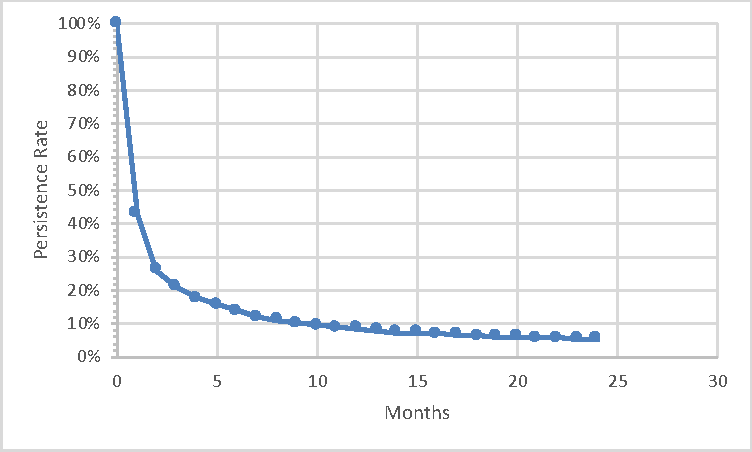
\includegraphics{figures/persistenceRateCrowdworks.pdf}
     \caption{Persistence Rate of Workers in CrowdWorks, according to the log of all workers who made accounts from January 1st, 2017 to December 31th, 2018.
     %\red{I hope this is okay to put in the paper. The figure needs to be improved. David: For the legend, maybe Persistence Rate of Workers on Crowdworks (50 workers, year 2019)? }
     }
     \label{fig:persistenceRate}
 \end{figure}

In December 2019, we conducted a poll of crowd workers on AMT and CrowdWorks, that have different characteristics; AMT is a microtask-based crowdsourcing platform, and CrowdWorks provides a wide variety of task types, focusing on a a bit larger tasks such as writing articles and codes.
This involved 101 workers (51 AMT and 50 CrowdWorks workers).
 Figure \ref{fig:surveyresult1}  summarizes the answers to the following questions: (Q1) Do you envision switching between platforms in the next X months? (Q2) How easy/challenging is switching between the platforms? 
 The result clearly shows that there is a strong correlation between worker mobility and the easiness of switching between platforms.
 We assume that since AMT is a pure microtask platform and obtaining a good reputation is easier, more workers think switching is easy in AMT than in CrowdWorks.
 Figure \ref{fig:surveyresult2} shows that workers would like platforms to have many advanced features that are not necessarily fully supported by the current generation of platforms. It is interesting to see that many workers on CrowdWorks dislike the collaboration feature among workers. We have not pursued the reasons yet, but a possible cause is the difference in the granularity of tasks. 

\begin{figure}[t]
\centering
\begin{tabular}{|c|c|c|c|c|c|c|c|}
\hline
Q1&Platform&\multicolumn{5}{|c|}{Q2}&Total\\
\cline{3-7}
&&Very Easy & Easy& Neither & Difficult & Very Difficult&\\
\hline
Yes&AMT&14\%&47\%&12\%&0\%&0\%&73\%\\
&CrowdWorks&0\%&2\%&6\%&2\%&0\%&10\%\\
\hline
No&AMT&4\%&6\%&6\%&10\%&2\%&26\%\\
&CrowdWorks&6\%&18\%&48\%&16\%&2\%&90\%\\
\hline
\end{tabular}
\caption{Results of Questions 1 and 2. The result suggests a correlation between the worker mobility  and the easiness of switching among crowdsourcing platforms.}
\label{fig:surveyresult1}
\end{figure}

\begin{figure}
    \centering
\begin{tabular}{|l|c|c|c|c|}
\hline
Q3. Preference for the feature?&Platform&\multicolumn{3}{|c|}{Answers}\\
\cline{3-5}
&&Like&Dislike&I don't know\\
\hline
Displaying Credentials&AMT&90\%&4\%&6\%\\
\cline{2-5}
&CrowdWorks&62\%&20\%&18\%\\
\hline
Specifying/ Quantifying/ Learning Skills&AMT&86\%&6\%&8\%\\
\cline{2-5}
&CrowdWorks&68\%&18\%&14\%\\
\hline
Anonymity&AMT&75\%&18\%&10\%\\
\cline{2-5}
&CrowdWorks&66\%&18\%&16\%\\
\hline
Complex Workflows&AMT&67\%&20\%&14\%\\
\cline{2-5}
&CrowdWorks&42\%&12\%&46\%\\
\hline
Collaboration&AMT&84\%&4\%&12\%\\
\cline{2-5}
&CrowdWorks&28\%&42\%&30\%\\
\hline
\end{tabular}
    \caption{Whether workers would like platforms to support for the features or not}
    \label{fig:surveyresult2}
\end{figure}

%\red{TBD after we get the poll results.}

%!TEX root = ../main.tex

% Abstract: we conclude the benefits in each period and give future challenges

% 


\begin{figure*}[!t]
\centering
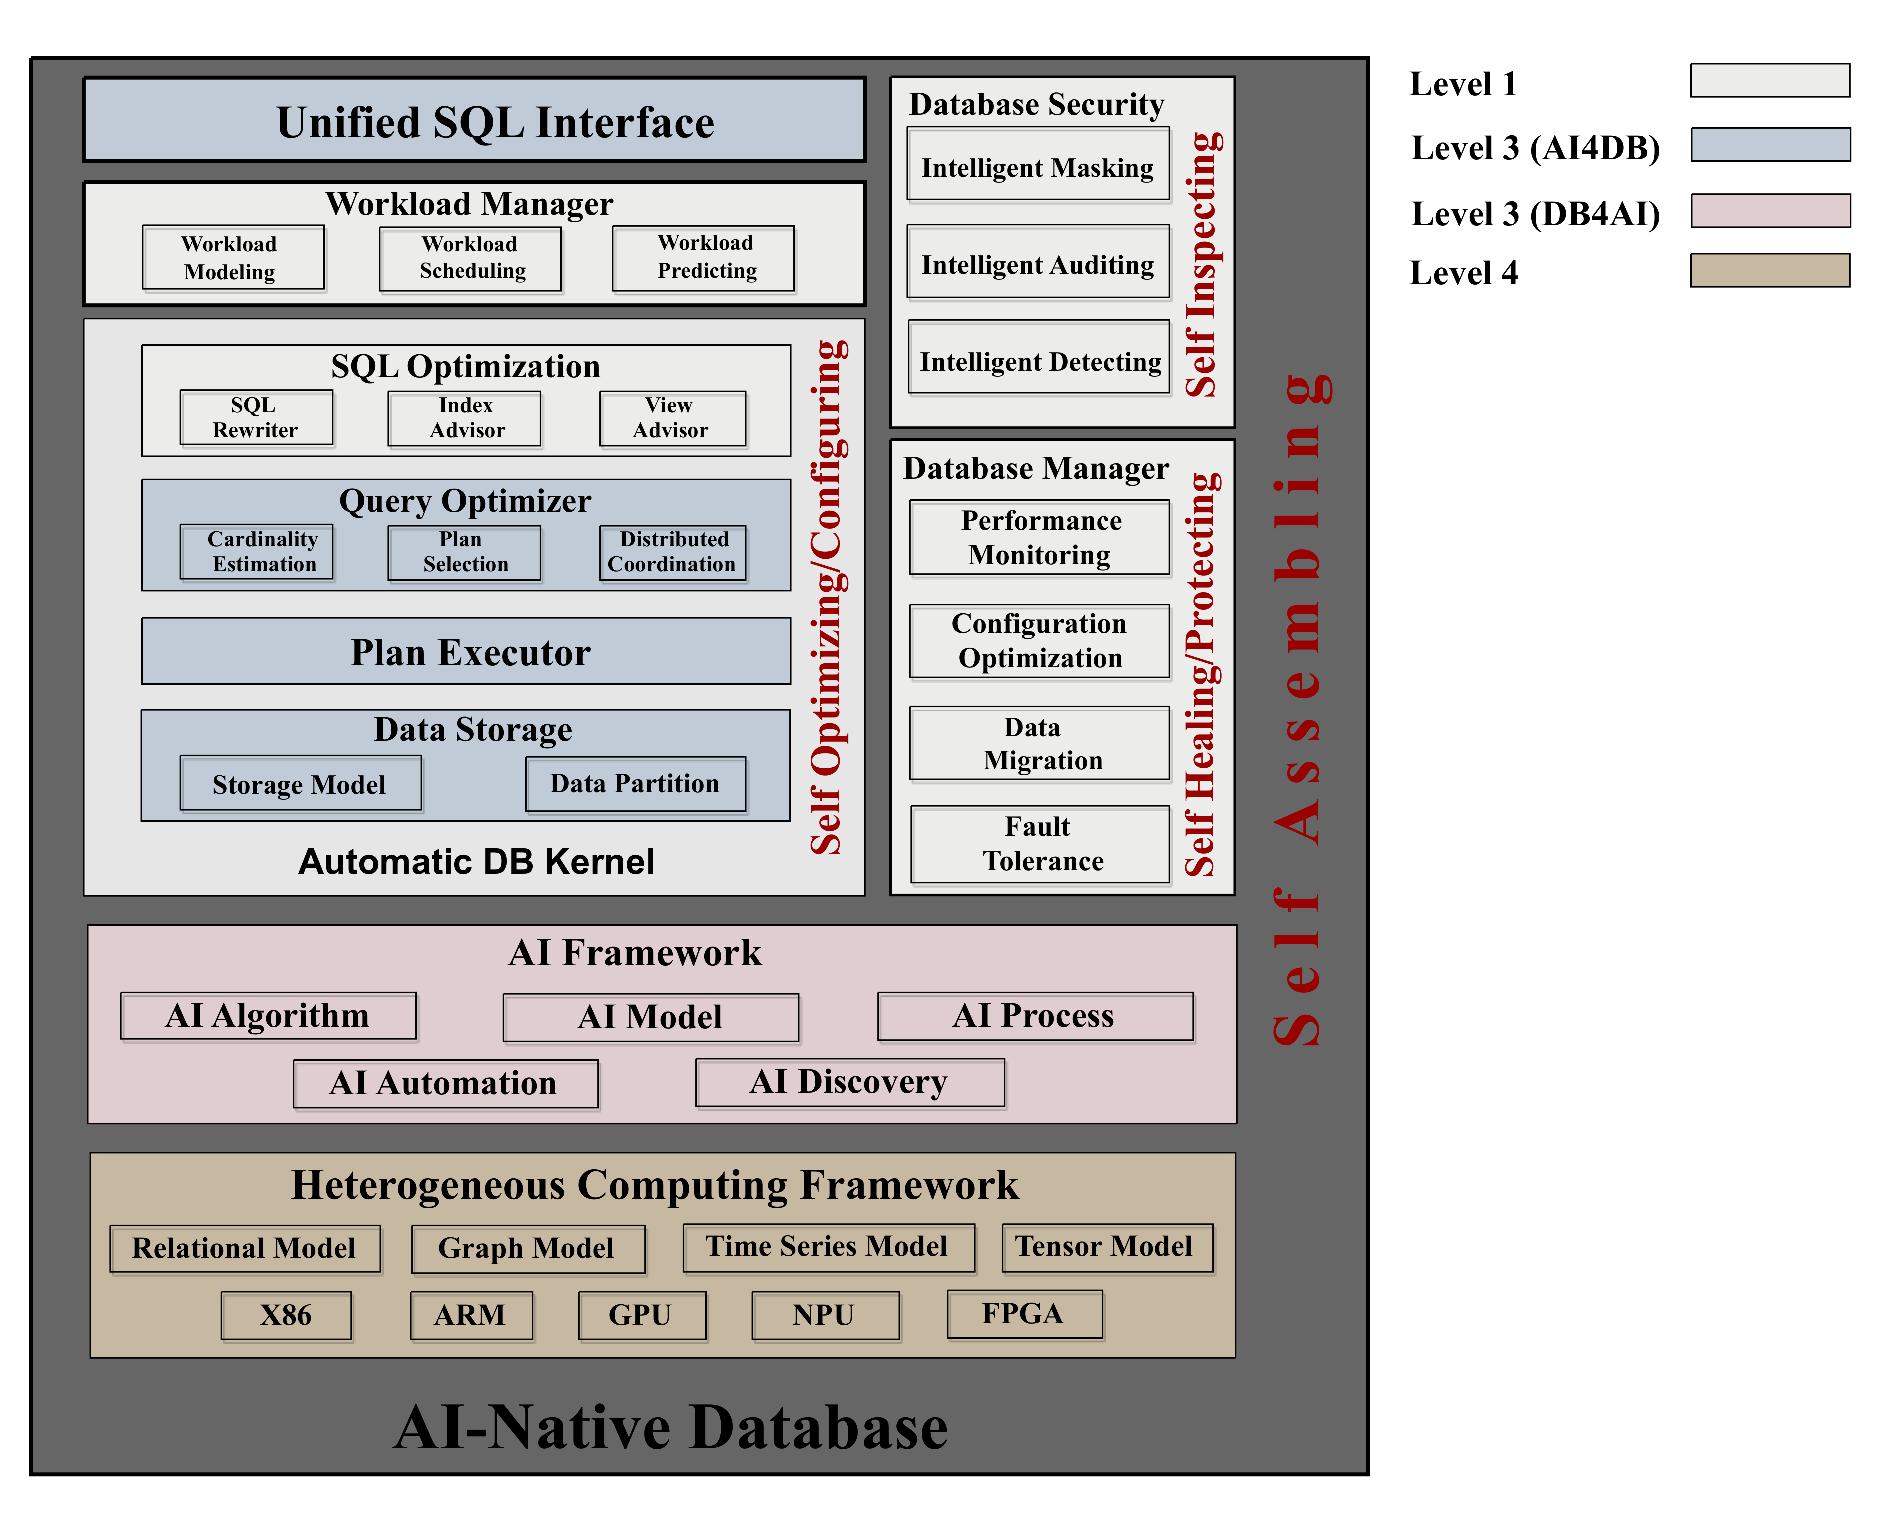
\includegraphics[width=1.0\textwidth, height=0.92\textwidth]{figs/ANDB-arch.eps}
\vspace{-1em}
\caption{The architecture of AI-Native databases}
\label{fig:ANDB}
\vspace{-1em}
\end{figure*}

 
To alleviate the issues talked above, in this section we propose a design of AI-native database, which better provides DB and AI services in five levels. 


\subsection{Level 1: AI-Advised Database}
\label{subsec: advised}
As shown in Table~\ref{tbl:ANDB}, in the first level, our database is AI-Advised, which provides auxiliary optimization of the database through suggestions~\cite{DBLP:conf/sigmod/AkenPGZ17, DBLP:journals/corr/abs-1802-00884, DBLP:conf/vldb/qtune19}.
It has an AI engine packing AI tools, which are loosely coupled with database in the form of plug-in. Limited by available resources, the AI engine mainly provides auxiliary tools from four aspects. 

$\circ$ \textbf{Workload Management}. It has two functions: to schedule user workloads and summary workload characters for the other modules. 
For \texttt{workload modeling}, traditional cost models are mostly based on empirical formulas, which have poor adaptability to different physical environments. Therefore, the machine learning model can be used to analyze and evaluate the current workload situation and future overhead, and dynamically adapt to the external environment based on gradient changes.
For \texttt{workload scheduling}, in traditional databases, resource scheduling depends heavily on parameters related to resource control, such as workspace size, maximum concurrent IO number, and etc. But these parameters are static and need to be manually configured. So we can use reinforcement learning to learn relations between database state (physical/logical), workload and database resources, and provide a reasonable and robust scheduling mechanism.
For \texttt{workload predicting}, workload usually dose not change in a fixed pattern. Traditional workload predicting methods are usually grasped by database experts according to statistical data, which can not guarantee high accuracy. So we proposed to use machine learning method for workload forecasting~\cite{DBLP:conf/sigmod/MaAHMPG18}, which can have better adaptability to different workloads. 
%In order to avoid using CPU, IO and other system resources as workload metrics in different hardware environments, we use logical metrics to characterize workload, which further ensures the stability of prediction.

$\circ$ \textbf{SQL Optimization}. It is to optimize database in SQL level. 
For \texttt{SQL rewriter}, SQL rewriter helps optimizer to choose efficient query plans by changing the way SQL is written. This level is often completed manually, which is impractical for heavy workload. So we provide a rewriting tool to learn the principles of SQL writing (e.g., avoiding full table scanning, selecting indexed columns as joins, and using table variables) and optimize the SQL structure. 
For \texttt{index advisor}, index is very important to improve the efficiency of retrieval tasks on complex data sets~\cite{DBLP:journals/kais/GaniSSH16}. However, the commonly used indexes are universal data structures. They do not analyze and utilize the distribution of data. So through machine learning, we can learn a model that reflects data patterns, and can automatically synthesize a special index structure at a lower cost.
For \texttt{view advisor}, given a set of queries, extracting high-frequency sub-queries and establishing materialized views to improve the performance of the database is very helpful. 
The traditional method caches at the whole query level, and the hit rate is low.
We construct the ML algorithm of sub-query selection according to the actual constraints so as to improve the query efficiency of batch SQL tasks.

$\circ$ \textbf{DB Manager}. It provides services (e.g., performance monitoring, tuning, fault tolerance) to ensure the stable operation of the database. In distributed scenario, high load pressure will lead to a sharp increase in failure rate, which brings great challenges to database maintenance. 
For \texttt{performance monitoring}, it automatically monitors the status of the database system (e.g., the number of batch requests per second, the number of user connections, network transceiver efficiency). Then it analyzes those indicators using machine learning algorithms. 
%Generally speaking, it includes four kinds of methods: real-time monitoring, timing monitoring, analysis report, tracking and data collection. Performance monitoring is not only statistical indicators, but also needs to understand the operation of the system based on these indicators. 
For \texttt{tuning}, database configuration involves hundreds of tunable system parameters, which control the database components in many aspects. Traditional tuning methods~\cite{DBLP:journals/pvldb/DuanTB09, DBLP:conf/cloud/ZhuLGBMLSY17} either relies on human beings (DBA-based), or cannot utilize history information (search-based). So we use a deep-reinforcement-learning-based tool~\cite{DBLP:conf/vldb/qtune19} to learn relations between database state, query and parameters, which can adapt to environment changes dynamically.
For \texttt{fault tolerance}, it includes a variety of strategies for resolving failures of hardware, transactions and system. In case of data error, the system needs to cancel the corresponding transactions in time. So we use a ML-based tool to monitor the changes caused by typical failures and realize pre-alerts. 

$\circ$ \textbf{DB Security}. It is to combine information security, cryptography technology with AI tech to  ensure the security of database. 
For \texttt{intelligent masking}, it is to hide privacy data such as ID number.  Intelligent masking technology only uses the high-dimensional, non-linear data inside the neural network to help improve the effect of data hiding. For example, in the research project conducted by Stanford University and Google, satellite images have been converted into high-frequency signals that are not easily detected. 
For \texttt{intelligent auditing}, it optimizes the auditing work from two aspects: data preprocessing and dynamic analysis. Traditional audit work often requires auditors to obtain a large number of business data. This part of the data understanding work is a waste of human resources. Intelligent auditing not only saves manpower cost, but also helps auditors to make better decisions by providing useful information from massive data.  
For \texttt{intelligent detecting}, it can automatically detect system vulnerabilities. Known intelligent detecting technology is mainly to retrieve through security scanning, while unknown security vulnerabilities need to do a lot of retrieval and testing work.  Using machine learning algorithm to discover security vulnerabilities~\cite{DBLP:journals/corr/abs-1902-10680}, it can not only detect most known vulnerabilities in national vulnerability database, but also predict and evaluate potential vulnerabilities.

\subsection{Level 2: AI-Assisted Database}
\label{subsec: assisted}
In the second level, our database is AI-Assisted, which is embedded into the database kernel for runtime optimization. AI components (e.g., tuning model, workload scheduling, view advisor)  can be merged into the corresponding database components~\cite{DBLP:journals/corr/abs-1903-01363}. This way, AI processes are integrated into the working procedure of the database. For example, if embedding the tuning model into the query optimizer, every time we generate the query plan, we can first conduct query tuning (adjust user-level parameters to better adapt to the incoming query characters), and then normally generate and execute query plan. The advantage of AI-Assisted database is that 1) it can provide more fine-grained optimization; 2) by embedding AI engine into the kernel, it can reduce much overhead such as communication cost.

However, neither Level 1 or 2 is a real AI-native database. Because the main components and organizing mode in those databases are still based on traditional methods. There are huge gap between AI technologies and databases. Starting from the third level, we introduce how to integrate intelligence integration, heterogeneity into database design to achieve the AI-native database.

\subsection{Level 3: AI-Enhanced Database}
\label{subsec: enhanced}
In the third level, our database is AI-Enhanced, which embeds intelligence and integration into database design. 
Firstly, we propose an intelligent database kernel, which implants AI into the design of database kernel. Secondly, we propose a  unified engine for both AI and DB, with which clients can use AI as easily as they use a DB.

\subsubsection{Intelligent Database Kernel}
\label{subsubsec: intelligent}
We present the design of an intelligent database kernel that enables self-configuring, self-healing, self-optimizing, self-protecting, self-inspecting and finally achieves self-organizing.

$\circ$ \textbf{Self-configuring}. Database can automatically adjust their own configuration to adapt to environment changes, including tuning parameters, upgrading software,adjusting partitioning/replication scheme, reorganizing tablespace and etc. Each function is embedded into particular DB modules to work as part of the processing.  For example, to realize tuning in query level, we embed tuner into optimizer. Each time a parse tree is input into our optimizer, it first configures parameters based on the query features and then actually generates the query plan. This way, it not only helps to generate better query plan, but prepares suitable environment for executing the query plan. 

$\circ$ \textbf{Self-healing}. Database can automatically detect, diagnose, alert and recover from DB problems (e.g., poor performance, hardware/software failovers). It adopts advantages of tools in AI-Advised DB to fully save humans from the failure-recovery loop. Firstly, it takes protective actions ahead of time (e.g., backup, data sharding, reosurce scheduling). Secondly, it can recover services even if emergency occurs (e.g., live migration).


%For example, rather than cleaning dirty pages in memory every fixed time, we replace the timing part  with the results of workload forcasting, which can predict how the workload varies. And it conducts cleaning when DB is free.live migration, checkpoint,  logging each write operations, we can focus on recording 

$\circ$ \textbf{Self-optimizing}. Database can automatically collect statistics of queries and optimize database performance in multiple granularities. Firstly, it collect statistics used in optimizer to learn current workload, which can benefit from cardinality estimation and workload scheduling. Secondly, it automatically design index, materialized query table (MQT) and data partition, which can directly optimize performance of single query. Thirdly, it automatically controls the flow of queries with query patroller to achieve overall optimization.

$\circ$ \textbf{Self-protecting}. Database can automatically monitor processing procedure of each query and prevent potential damage in time. For example, it can throttle service requests which compete resources to cut down deadlock and average waiting time; and it can kill / lower the priority of run-away queries (execution time is far longer than that estimated by the optimizer) to prevent from using up system resources.

$\circ$ \textbf{Self-inspecting}. Database can automatically monitor database state and conclude operating rules by itself. It can check database state (e.g., data consistency, DB health) all the time. And by concluding all the failover conditions and solutions, it can translate the experience in the form of publication of instrumentation data in favor of human understanding.


$\circ$ \textbf{Self-organizing}. For current databases, each level of service (e.g., parser, optimizer and executor) has multiple standardized components to choose from. How to choose the appropriate processing path for one or a batch of queries becomes meaningful. 

So we propose a self-organizing module. For different queries, we can dynamically select the appropriate components in each layer of service and assemble the appropriate execution path.
The execution path can be seen as a natural language sequence (NLS), such as $\langle$ $SQL_i$, parser$\_$pg, optimizer$\_$RBO, storage row, accelerator $\rangle$, in which each position has only discrete token options. So the problem is how to generate NLS in query level. One method is to use RL algorithm. It takes the whole path sequence as an episode and a single action as an epoch. Under each epoch, the agent chooses the next component (action), which executes the query, leading to a state transition (e.g., the query status changes into syntax tree). In this problem, action is discrete, so DDQN algorithm~\cite{DBLP:conf/aaai/HasseltGS16} can be used. Compared with other RL algorithms with discrete output, DDQN eliminates the problem of overestimation (deviate greatly from the optimal solution) by choosing decoupling actions and calculating the target Q value.

However, RL-based routing algorithm has two problems. 
Firstly, Q network will not score until the last node is generated. It is insensitive to the choice of intermediate nodes. However, for the entire path, it is necessary to give action a comprehensive score on current and future impacts. 
Secondly, when training with epoch as a unit, each node of a path is scattered in a training sample, instead of being used as a whole to calculate the gradient. 

Generating antagonistic network (GAN)~\cite{DBLP:journals/corr/abs-1902-05687} can better solve those problems of end-to-end path selection. We use G network to generate path vectors based on workload, database state and component characteristics, and we use D network as the performance model. 
But the traditional GAN network model is not fully applicable to our problem. Because it is mainly used to generate data with continuous range of values, and it is difficult to generate path vectors with discrete tokens. That is because G-networks need to be fine-tuned based on gradient descent and regress towards the expectation. But when the data is discrete tokens, fine-tuning is often meaningless.
So we choose to combine RL algorithm with GAN~\cite{DBLP:conf/aaai/YuZWY17}. Firstly, G network is used as agent in RL algorithm: action is the next service node; state includes not only query status, database status, but also generated node information. Each iteration generates a complete path. Secondly, unlike pure RL algorithm, each action is scored by D network to guide the generation of the whole path sequence.

\subsubsection{Unified Engine for AI and DB}
\label{subsubsec: engine}
After achieving the intelligent database kernel, we gain real integration by providing unified engine for DB and AI. AI and DB are closely connected. For DB, as talked above, AI can make DB  smarter. For AI, DB stores large scale of data for training the ML models. 
So it becomes easy when we can call ML model with SQL statements. Firstly, SQL is easy to use, with which technicians with basic SQL knowledge can complete most of traininig and predicting tasks. Secondly, it saves people from frequently switching between different languages of systems, when we need to write SQL to fetch data and run python scripts to run ML algorithms.

For this work, there have been some products such as BigQuery ML~\cite{DBLP:conf/ideas/FernandesB15}, SQL for DL and SQLFlow. Considering the Pros and Cons of these works, we propose an extended DB engine to achieve the following aims:

$\circ$ \textbf{AI Support}. Firstly, SQL Parser should extend SQL syntax to utilize AI methods, including model creating, training and predicting. Besides, it should minimize the use of other scripting languages (e.g., Python and R). Secondly, we extend the relational algebra theory to support both relational and tensor data models. This way, DB can support tensor processing, which is largely used in the training of AI models.


$\circ$ \textbf{General Purpose}. SQL parser should contain an abstract layer which maintains a loose couple with lower components. This way, it can be easily used on different SQL engines (e.g., PostgreSQL, Flink and Hive) or machine learning toolkits (e.g., TensorFlow, Keras and scikit-learn). 

$\circ$ \textbf{Custom Style}. Besides general operators such as SELECT and WITH, we also allow user to define how to train, evaluate and predict the ML models with user-defined functions. And they also can cache the trained model with materialized views.

The general workflow is as follows. Firstly, SQL Parser parses a SQL statement and produces a general-purpose query plan. Based on the operators in the plan, it decides whether it is for manipulating data or calling ML models. If for manipulating data, the query plan is sent to the DB executor and be executed. Otherwise, it is sent to the AI executor and be executed.

This way, database can also provide AI services in an end-to-end way. As table~\ref{tbl:AI} shows, Database supports AI services in five levels.
%Presently, DB mainly serves for structured data analysis such as financial transactions. By embedding AI algorithms into DB engine, DB can directly support many AI applications (e.g., image comparison, graph computing) in an end-to-end way. As Figure~\ref{fig:DB4AI} shows,  

$\bullet$ \textbf{DB-based AI Algorithm}. Database provides ML tool-kits and libraries (e.g., TensorFlow, Scikit-learn). Clients can write AI algorithms in UDFs or stored procedures. And they can call them repeatedly from database. 

$\bullet$ \textbf{DB-based AI Model}. Database provides classic AI models (e.g., random forest, RNN, DDQN). Clients can directly call AI models from database and only focus on the training part. 

$\bullet$ \textbf{DB-based AI Process}. Database further provides AI processes, which not only include the mature AI models but the training methods (e.g., SGD, Adam, reinforcement learning). Clients can directly call AI processes from database, only with data as input. Database automatically fine-tunes AI model using corresponding training method, and utilizes the model to produce results. 

$\bullet$ \textbf{DB-based Automation}. Database can automatically parse the requirements in AI and call proper process to solve it. Clients only need to declare their requirement. For example, if we hope to search some images, we just declare the conditions and data sources with SQL. And database automatically chooses the CNN model to conduct the work, which is also a part of the query plan.

$\bullet$ \textbf{DB-based Discovery}. Database offers an insight into the data schema and application queries, and optimizes itself with AI techniques. For example, if a new workload comes, database can call a DRL-based tuner to adjust the system parameters based on the query features, including cost estimation, resource allocation, concurrency  control and etc. 

\begin{table}[h]
\vspace{-1em}
\centering
\caption{Five levels of machine learning consumability in DBMS}
\label{tbl:AI}
{%\footnotesize
  \hspace*{-0em} \begin{tabular}{|c|c|l|c|c|}\hline
  
\multirow{2}{*}{\textbf{Level}} & \multirow{2}{*}{\textbf{Consumability}} & \multirow{2}{*}{\textbf{\ \ \ \ \ \ \ \ \ \ \ \ \ \ \ \ \ \ \ \ \ \ \ \ Description}} & \multirow{2}{*}{\textbf{Target Users}} & $\textbf{ML Skill}$ \\
 &  &  & & $\textbf{Level}$ \\\hline

\multirow{2}{*}{\textbf{1}} & \multirow{2}{*}{Algorithm} & \multirow{2}{*}{Algorithms as UDFs and stored procedures} & Data scientists,  & \multirow{2}{*}{High} \\
 &  & & experienced developers & \\\hline


\multirow{2}{*}{\textbf{2}} & \multirow{2}{*}{Model} & Models as first-class object with DDL, & App. developers  & \multirow{2}{*}{Medium} \\
 &  &  DCL, DML capability  & and DBAs & \\\hline

\multirow{2}{*}{\textbf{3}} & \multirow{2}{*}{Process} &  Processes as first-class object with DDL, & App. developers & \multirow{2}{*}{Low} \\
 &  & with DCL, DML capability  & and DBAs & \\\hline

\multirow{2}{*}{\textbf{4}} & \multirow{2}{*}{Automation} &  Problem specifications as first-calss object & Business specialists, DBAs & \multirow{2}{*}{Low} \\
 &  & with DDL, DCL, DML capability  & app. developers & \\\hline


\multirow{2}{*}{\textbf{5}} & \multirow{2}{*}{Discovery} &  Discover ML opportunities based on & Business specialists, DBAs & \multirow{2}{*}{Very Low} \\
 &  & data schema and application queries  & app. developers & \\\hline

  
  \end{tabular}
}
\vspace{-1em}
\end{table}

\subsection{Level 4: AI-Assembled Database}
\label{subsec: assemble}
In the fourth level, our database is AI-Assembled, which embeds heterogeneity into database design. That is ,we assemble AI with database by supporting multiple leading computing powers. We know traditional database is only based on CPU. However, DB and AI technology usually require different computing power and hardware. For DB, traditional optimizer processes queries with CPU. While AI technology requires new chips to support parallely processing (e.g., GPU and NPU) and self-scheduling. And now many applications need to use both DB and AI technology, especially in large data analysis scenarios.

AI-assembled database mainly has two contributions. Firstly, it can support ARM architecture. 
1) It effectively utilizes ARM array with multi-core mode, inter-node parallelism, intra-node parallelism, instruction-level parallelism, compiler parallelism and other super-parallel technologies. 
2) For the problem of competition brought by multi-core, it provides cross-chip access optimization and resource scheduling optimization. 
Secondly, it can utilize different computing powers to better serve the AI components. It is able to switch computing powers based on the processing types. For example, for the tuning module in optimizer, when training the tuning model, we fetch training data into memory with ARM and conduct backward propagation (training the neural network) with NPU. And database should flexibly schedule computing powers, e.g., when NPUs are overburdened but most ARM resources are idle, ARM array can share some burden.

The ultimate objective of this database is to fully unleash the power of diversified computing, which includes x86, ARM, GPU, NPU, and accelerators. We aim to continuously push our AI strategy forward and foster a complete computing ecosystem. 


\subsection{Level 5: AI Designed Database}
\label{subsec: designed}
In the last level, AI technology is integrated into the whole database life cycle (DBLC) of our database so as to achieve the ultimate goal of scenario-aware and AI-as-a-Service. The whole life cycle includes five phases: 1) Database initialization; 2) Database design; 3) Database implementation; 4) Database evaluation; 5) Database operation and maintenance.


\begin{table}[h]
\vspace{-1em}
\centering
\caption{Five levels of AI-native database}
\vspace{0.5em}

\label{tbl:ANDB}
{%\footnotesize
  \hspace*{-0em} \begin{tabular}{|c|c|l|l|}\hline
  
\multirow{1}{*}{\textbf{Level}} & \multirow{1}{*}{\textbf{Feature}} & \multirow{1}{*}{\textbf{\ \ \ \ \ \ \ \ \ \ \ \ Description}} & \multirow{1}{*}{\textbf{\ \ \ \ \ \ \ \ \ \ \ \ \ \ \ \ \ \ \ \ \ \ \ \ \ \ \ \ \ \ \ \ \ \ \ \ Example}} \\\hline

\multirow{4}{*}{\textbf{1}} & \multirow{4}{*}{AI-advised} & \multirow{4}{*}{ plug-in AI engine} &$\circ$ Workload Manager (e.g., \small{workload scheduling/predicting})  \\
 &  & & $\circ$  SQL Optimization \small{(e.g., SQL rewriter, index/view advisor)} \\
 &  & &$\circ$  DB Maintenance \small{(e.g., knob tuner, fault tolerance)}\\
 &  & &$\circ$  Security \small{(e.g., intelligent masking/auditing/detecting)}\\\hline

\multirow{4}{*}{\textbf{2}} & \multirow{4}{*}{AI-assisted} & \multirow{4}{*}{Built-in AI engine} &$\circ$ Embed workload scheduling as job-queue mechanism \\
 &  & & $\circ$  Embed index advisor as an optional database indexing\\
 &  & &$\circ$ Embed knob tuner as a self-adaptive module \\
 &  & &$\circ$  Replace database auditing with intelligent auditing \\\hline

\multirow{7}{*}{\textbf{3}} & \multirow{7}{*}{AI-enhanced} & \multirow{7}{*}{Hybrid DB\&AI engine} &$\circ$ Intelligent Database Kernel \\
 &  & &\ \ \  $\bullet$ Self-configuring (e.g., self tune/upgrade/data partition)\\
 &  & &\ \ \  $\bullet$ Self-healing (e.g., self failover/alert/recovery)\\
 &  & &\ \ \  $\bullet$ Self-optimizing (e.g., collect stats, design index/MQT)\\
 &  & &\ \ \  $\bullet$ Self-protecting (e.g., throttle run-away queries )\\
 &  & &\ \ \  $\bullet$ Self-inspecting (e.g., consistency/health check)\\
 &  & &\ \ \  $\bullet$ Self-organizing (e.g., form executing path in query level)\\
 &  & &$\circ$ Unified Engine for AI+DB \\\hline

\multirow{2}{*}{\textbf{4}} & \multirow{2}{*}{AI-assembled} & \multirow{2}{*}{Heterogeneous computing} &$\circ$ Support new hardware (e.g., ARM, GPU, NPU) \\
 &  &   &$\circ$  Extend relational algebra to support tensor model \\\hline

\multirow{5}{*}{\textbf{5}} & \multirow{5}{*}{AI-designed} & \multirow{5}{*}{The life cycle is AI-based} &$\circ$ Database initialization \\
 &  & & $\circ$  Database design\\
 &  & &$\circ$ Database implementation and loading\\
 &  & &$\circ$  Database testing and evaluation \\
 &  & &$\circ$  Database operation and maintenance \\\hline
  
  \end{tabular}
}
\vspace{-1em}
\end{table}




%!TEX root = ../main.tex

\section{Challenges and Opportunities}
\label{sec: challenge}

It brings new research challenges and opportunities to design an AI-native database, which aims to support data management, data analysis, machine learning together in the same system.

\subsection{From one-size-doesn't-fit-all to one-stack-fits-all}

Michael Stonebraker argues that one size does not fit all, due to various applications (e.g., OLTP, OLAP, stream, graph) and diversified hardware (e.g., CPU, ARM, GPU, FPGA, NVM). Note that the database components and their variants are limited, but the number of possible combinations for these components to assemble a database is huge. So the database architects design the database architectures by combining different variants of techniques based on their empirical rules and experience. Thus these human-designed databases may not be optimal because they may fall into a local optimum. It calls for automatically designing a database using AI techniques, which can adapt to different scenarios. 


We argue that one stack fits all. The basic idea is to first implement the database components, e.g., indexes, optimizers, storage, where each component has multiple variants/options, then use AI techniques to assemble these components to form some database candidates, and finally select a database that best suits a given scenario. In this way, we can automatically verify different possible databases (i.e., different combinations of components), explore many more possible database designs than human-based deign, and could design more powerful databases. This is similar to AlphaGO, where the learning-based method beats humans, because the machines can explore more unknown spaces. 


There are several challenges in one-stack-fits-all. First, each component should provide standard interfaces such that different components can be integrated together. Second, each component should have different variants or implementations, e.g., different indexes, different optimizers. Third, it calls for a learning-based component to assemble different components. Fourth, the assembled database can be evaluated and verified before the database is deployed in real applications.  Fifth, each component should be run on different hardware, e.g., learned optimizers should be run on AI chips and traditional cost-based optimizers should be run on general-purpose chips. It calls for effective methods to schedule the tasks. 


\subsection{Next Generation Analytic Processing: OLAP 2.0}

Traditional OLAP focuses on relational data analytics. However, in the big data era, many new data types have emerged, e.g., graph data, time-series data, spatial data, it calls for new data analytics techniques to analyze these multi-model data. Moreover, besides traditional aggregation queries, many applications require to use machine learning algorithms to enhance data analytics, e.g., image analysis. Thus it is rather  challenging to integrate AI and DB techniques to provide new data analytics functionality. We think that hybrid DB and AI online analytic processing on multi-model data should be the next generation OLAP, i.e., {\it OLAP 2.0}. 

There are several challenges in supporting OLAP 2.0. First, different data types use different models, e.g., relational model, graph model, KV model, tensor model, and it calls for a new model to support multi-model data analytics. Second, OLAP 2.0 queries may involve both database operations and AI operations, and it needs to design new optimization model to optimize these heterogeneous operations across different hardware. 



\subsection{Next Generation Transaction Processing: OLTP 2.0}

Traditional OLTP mainly uses general-purpose hardware, e.g., CPU, RAM and Disk, but cannot make full use of new hardware, e.g., AI chips, RDMA, and NVM. Actually, we can utilize new hardware to improve transaction processing. First, based on the characteristics of NVM, including non-volatile, read-write asymmetry speed, and wear-leveling, we need to reconsider the database architecture. For example, we can utilize NVM to replace RAM and replace page-level storage with record-level storage on NVM. Second, we can utilize RDMA to improve the data transmission in databases. Moreover, we can use the programmable feature of intelligent Ethernet card to enable filtering on RDMA and avoid unnecessary processing in RAM and CPU. Third, there are some AI chips which are specially designed hardware, and it is also promising to design database-oriented chips that are specially defined hardware for databases. 


There are several challenges in supporting OLTP 2.0. First, it is challenging to fully utilize new hardware to design a new generation database. Second, it is hard to evaluate and verify whether the new hardware can benefit the database architecture. Third, it calls for an effective tool to automatically evaluate a feature or a component (even a database). 




% Fifth, each component should be run on different hardware, e.g., learned optimizers should be run on AI chips and traditional optimizers should be run 




\subsection{AI4DB}

There are several challenges that embed AI capabilities in databases. 

\hi{Training Samples.} Most AI models require large-scale, high-quality, diversified training data to achieve good performance. However, it is rather hard to get training data in databases, because the data either is security critical or relies on DBAs. For example, in database knob tuning, the training samples should be gotten based on DBAs' experiences. Thus it is hard to get a large number of training samples. Moreover, the training data should cover different scenarios, different hardware environments, and different workloads.  

% Moreover, the training data must be high quality, number and diversity of samples.

\hi{Model Selection.} There are lots of machine learning algorithms and it is hard to automatically select an appropriate algorithm for different scenarios. Moreover, the model selection is affected by many factors, e.g., quality, training time, adaptability, generalization. For example, deep learning may be a better choice for cost estimation while reinforcement learning may be a better choice for join order selection. The training time may also be important, because some applications are performance critical and cannot tolerate long training time. 

%, which usually cannot be satisfied in database. Second, any AI model needs relatively long training time, which is usually intolerable in database.

\hi{Model Convergence.} It is very important that whether the model can be converged. If the model cannot be converged, we need to provide alternative ways to avoid making bad decisions. For example, in knob tuning, if the model is not converged, we cannot utilize the model for knob suggestion.   
 
\hi{Adaptability.} The model should be adapted to different scenarios. For example, if the hardware environments are changed, the model can adapt to the new hardware. 
  
\hi{Generalization.} The model should adapt to different database settings. For example, if the workloads are changed, the model should support the new workloads. If the data are updated, the model should be generalized to support new data. 
 

\subsection{DB4AI}

\hi{Accelerate AI algorithms using indexing techniques.} Most of studies focus on the effectiveness of AI algorithms but do not pay much attention to the efficiency, which is also very important. It calls for utilizing database techniques to improve the performance of AI algorithms. For example, self-driving vehicles require a large number of examples for training, which is rather time consuming. Actually, it only requires some {\it important examples}, e.g., the training cases in the night or rainy day, but not many redundant examples. Thus we can index the samples and features for effective training. 


\hi{Discover AI Models.} Ordinary users may only know their requirements, e.g., using a classification algorithm to address a problem, but do not know which AI algorithms should be used. Thus it is important to automatically discover AI algorithms. Moreover, it is also challenging to reuse the well-trained AI models by different users. 



\subsection{Edge Computing Database.} Most databases are designed to be deployed on servers. With the development of 5G and IOT devices, it calls for a tiny database embedded in small devices. There are several challenges in designing such a tiny database. The first is database  security to protect the data. The second is real-time data processing. The small device has low computing power, and it is rather challenging to provide high performance on such small devices. The third is data migration among different devices. Some devices have small storage and it is challenging to migrate the data across different devices. 



%\hi{Security}

%\hi{Database function As a Service}



%, and deploy the  automatically designed database for different .  

%Note that different databases usually adopt the common techniques, e.g., index and cost-based optimizer, but 

%The database architects 
%As Figure~\ref{fig:ANDB} shows, AI-native database can support AI and DB services naturally and efficiently. It brings new opportunities to the development of database. However, due to the demands of AI algorithms (e.g., training data), as well as problems in DB technology itself, there are still several challenges in the process of deploying such a design.

%\subsection{Challenges in AI}
%\label{sec: ch-AI}
%Challenges in AI is mainly around two aspects. First, any AI model needs large-scale and high-quality training data to achieve good performance, which usually cannot be satisfied in database. Second, any AI model needs relatively long training time, which is usually intolerable in database.

%\subsubsection{Lack of training data}
%\label{subsec: data}
%AI algorithms rely on training data heavily, including the quality, number and diversity of samples.

%$\bullet$ \textbf{Sample Quality}. Sample quality has the most direct impact on the quality of model training. In order to train the prediction model correctly, the sample data must be correct and de-duplicated. But it is difficult to guarantee the data quality in the database system. Firstly, although the database system has abundant statistical information, many of these information are not real-time updates, such as the statistical information of relational tables. Secondly, these data will be affected by many factors, such as cardinality estimation, not only the data distribution information of relational tables, but also the execution cost of various physical operations of the database.

%$\bullet$ \textbf{Sample Number}. High quality samples alone are not enough to train robust AI models. Taking neural network as an example, if the training samples are very small and the number of updates of connection weights is small, the space that the model can explore is very limited. And the adaptability of the model can be weak. While in DB, many problems can hardly provide enough training samples. For example, for workload forecasting, user data in real scenarios are often hard to get, under strict protection.

%$\bullet$ \textbf{Sample Diversity}. Although the mature machine learning model can adapt to new problems, providing typical samples in training stage can accelerate the convergence speed of the model and improve the accuracy and adaptability of the model. However, in database-related problems, due to the limited training time allowed, it is often difficult to obtain sufficient and diverse data in the initial training stage. For example, in the tuning problem, the training stage often only provides several typical benchmark workloads.

%\subsubsection{Unaffordable Training Time}
%\label{subsubsec: time}
%Data alone is not enough for machine learning. The learning model needs enough training time to transform input knowledge into output knowledge. Therefore, in fact, simple classifiers can be widely used, because training complex classifiers takes a long time. Similarly, it is difficult for database systems to converge when they are faced with various user needs. Therefore, there are two requirements for the selection of machine learning algorithm in database system. First, the model adapts to the scenario. For example, in tuning problem, many parameters have continuous ranges of values, and algorithms such as Q-learning need to keep large-scale tables, which wastes time and resources. Secondly, it combines gradient descent and transfer learning to improve training efficiency. Up to now, many algorithms have been proposed to optimize training efficiency. For example, in reinforcement learning, Actor-Critic algorithm can enhance the convergence speed with the Critic evaluating the behavior of the Actor.

%\subsection{Challenges in DB}
%\label{sec: DB}
%Here we mainly consider the challenges that DB can bring about to AI. There are three problems.

%\subsubsection{Various Hardware}
%\label{subsec: hardware}
%The challenges of the hardware environment include two aspects. 

%$\bullet$ Hardware on which database processes transactions. New computing and storage media are emerging, with ROM like  SSD, disk array, NVM and CPU architectures like SMP, AMP. People often configure different for thier databases, considering many factors (e.g., budgets, applications). And in cloud environment, much more hardware instances exist. Different hardware environments can have a great impact on AI technology. For example, in knob tuning, many parameters are strongly related to hardware, such as the cost of reading/writing tuple, the overhead of database operators and so on. The model will take a long time to correct the historical cognition without taking the hardware changes into consideration. 
%For example, in cardinality estimation technology, if the system supports multiple threads (workers) to execute a query plan in parallel, the relationship between operator overhead at different levels is no longer simple summation. Machine learning model needs more time to adapt to the change of implicit rules. 

%$\bullet$ Hardware on which AI model is trained. In order to reduce the time used to train large-scale machine learning models, Intel, Google, Microsoft and other manufacturers have released a variety of hardware specifically to help train AI models (e.g., GPU, TPU, FPGA). Altough those hardwares improve the efficiency of matrix computing, they require the corresponding adjustment of machine learning algorithm to adapt. For example, For example, if you want to migrate an AI model from CPU to GPU, you need to migrate tensors, variables and the model to the display memory in GPU.

%\subsubsection{Various Workload}
%\label{subsec: workload}
%Various workloads pose challenges in two aspects.

%$\bullet$ With different workloads, the database not only needs to provide appropriate operation and maintenance strategy, execution plan, processing flow, but also needs to provide appropriate architecture to store data. For example, in edge computing, we need to provide services nearby, and there are some problems such as data/service migration; in cloud database, it manages data uniformly and maintains diverse distributed clusters. Firstly, that requires AI model to filter out the important factors in the workload, and dynamically adapt to changes. 

%$\bullet$ Hybrid application services increase the complexity of database management.  Different workload types often correspond to different services, such as OLTP, OLAP and HTAP. And many applications require hybrid services. For example, banking system not only provides transactional business, but also needs analytical business such as data auditing and analysis. So database instances can no longer serve one type workload. This kind of composite business has higher requirements for database storage, processing and data management. This requires that the machine learning model trained from a single scenario can provide a good enough service for hybrid workload types.

%\subsubsection{Various User Requirements}
%\label{subsec: requirement}

%Different users often notice different database performance. For example, real-time services require low query latency, while batch services require high throughput. In order to guarantee the desired performance, databases often need to sacrifice the performance of other aspects. For example, in order to improve the utilization of the overall resources, the number of parallel connections can be increased, but the workspace allocated for each connection will be reduced, which will affect the execution efficiency of a single task. In cloud databases, there are a variety of user "preference". In order to use machine learning to optimize database technology, it is necessary that machine learning model can automatically and quickly adapt to the requirements of different users, and allocate resources reasonably based on priority. 
%And use various statistical, caching, data collation mechanisms (such as vacuum) to improve resource utilization and fault-tolerant disaster prevention capabilities, improve resource utilization and database stability, and further enhance user experience.




\section{Conclusion}\label{sec:conclusions}
Alternative job arrangements such as online job platforms are becoming increasingly important
and a major source of employment in the near future.
It is important for the crowdsourcing community to take the lead on researching the Feature of Work.
In this article, we argue that a key pre-requisite is the creation of benchmarks for such research.
The diversity of crowdsourcing research by various communities is a key challenge.
We propose a taxonomy of dimensions for which benchmarks has to be developed.
We also have enumerated a list of metrics that are most relevant for effective crowdsourcing. Moreover, we list essential factors that need to be considered during the process of creating benchmarking data to test the effectiveness and robutness of crowdsouring platforms. Benchmarks have had a dramatic impact in the development of various domains.
We issue a call-to-arms to the crowdsourcing community to seize the opportunity!

%%!TEX root = ../main.tex

\section{QUERY Clustering}
\label{sec:cluster}

For workloads including both transactional queries and analytical queries~\cite{DBLP:conf/icde/OhL05}, if the user aims to optimize the latency, we recommend  {\it query-level} tuning; if the user aims to improve the throughput, we recommend  {\it workload-level} tuning. For analytical only queries, we recommend cluster-level tuning to balance the throughput and latency. The key problem in the cluster-level tuning is (1) how to efficiently find the appropriate {\it configuration pattern} for each query and (2) how to cluster the queries based on the configuration pattern.  This section studies these two problems. % in this section.


\subsection{Configuration Pattern}
\label{sec:pattern}
The configuration pattern of a query should include all the knobs used in the DS-DDPG model. Thus a nature idea is to use DS-DDPG to generate a continuous knob configuration and take the knob configuration as the pattern. However it is rather expensive to get the continuous knob values, especially for a large number of queries. More importantly, when we cluster the queries, we do not need to use the accurate configuration pattern; instead approximate patterns are good enough to cluster the queries. 

\lgl{To this end, we discretize the continuous values into discretized values. For example, we can discretize each knob into \{-1,0,+1\}. Specifically, for each knob, if the tuned knob value is around the default value, we set it as 0; 1 if the estimated value is much larger than the default value; -1 if the estimated value is much smaller than the default value.}

\lgl{To avoid the curse of dimensionality when clustering queries, we only choose knobs most frequently tuned by DS-DDPG as the features, about 20 in PostgreSQL.} But the new knob space is still very large. For example, if \lgl{20} knobs are used and each has 3 possible values, then there are $3^{\lgl{20}}$ possible cases. The traditional machine learning methods or regression models are hard  to solve this problem, because they either assume the labels are independent such as Binary Relevance~\cite{DBLP:journals/pai/LuacesDBCB12} or cannot support so many labels such as Classifier chain~\cite{DBLP:journals/ml/ReadPHF11}. 



\vspace{.25em} 
\noindent {\bf  Learning Discrete Configuration Patterns Using Deep Learning.}  We choose the deep learning method to map queries to discrete configuration patterns. As Figure \ref{fig:DL} shows, the \texttt{Vector2Pattern} uses a neural network, which adopts a five-layer architecture. 

The input layer takes the feature vector as input and maps it to the target knob space, in order to make the input and output in the same scale. 

The second layer is designed to explore the configuration patterns. It is a dense layer with \lgl{ReLU} as the activation function %It expends the feature space by 2 times to explore more complex patterns. And  \lgl{ReLU}  
$(y = max(x, 0)$, where $x$ is an input feature and $y$ is the corresponding output features, using to learn two aspects of knowledge: 1) Interaction effects; 2) Non-linear effects. Interaction effects capture the correlations among the input features. For example, feature $v_i$ captures the value difference when other features' value changes. While Non-linear effects learns non-linear mapping relations between input vector and output vector. 

The third layer is a BatchNormal layer. It normalizes the input vector in favor of gaining discretized results. 

The fourth layer has the same function as the second and the value of each feature in this layer's output vector ranges from 0 to 1. But different from \texttt{Predictor} in Section~\ref{sec:tunner}, the last layer uses a {\it sigmoid}  activation function $S(z_{i})$ = $\frac{1}{1+e^{-z_{i}}}$, where $z_i$ is the $i_{th}$ feature of the input vector. It takes a real value as input and outputs a value in 0 to 1. This aims to do a non-linear data transformation and  at the same time keeps the features in the limited range.  

%\lgl{It is nonlinear, continuously differentiable and it changes monotonously.}  % To avoid sparing space causes too many $"$noise$"$ points, we also convert the knobs of numerical type into discrete values. 

For the DL model, we also append a step function to the network's end and use the output layer as a probability distribution function: for each feature $y$ in the output vector, the resulting bit is -1 if $y$ is below 0.5; 0 if $y$ equals to 0.5; and 1 otherwise. In this way, the DL model can automatically finish data transformation and discretization work. 

%\lgl{what is y?}\lgl{give more details of deep learning model!!!}


\begin{figure}[!t]\centering
\vspace{-.5em}
\includegraphics[width=.45\textwidth, height=.27\textwidth]{tuning_figs/DL_x.eps}
\vspace{-2em}
\caption{Architecture of the DL model}
\label{fig:DL}
\vspace{-2.5em}
\end{figure} 


\vspace{.25em} 
\noindent{\bf Workflow of \texttt{Vector2Pattern}.} 
The DL model works in 4 steps: 1) For each training sample $\langle q, p_r\rangle$, where $q$ is a query and $p_r$ is the real pattern that matches $q$,  compute the feature vector $v$ of query $q$; 2)  Propagate these features through its network; 3) Output an estimated  pattern $p_e$; 4) Based on the output pattern $p_e$ and the actual pattern $p_r$, update the weights in the network by minimizing $|p_e-p_r|$. 



\vspace{.25em} 
\noindent{\bf Training Step. } We need to generate a large volume of samples to train \texttt{Vector2Pattern} until the performance on a new testing set is good enough (i.e., high generalization ability). Each training sample is in the form of $\langle q, p\rangle$, where $q$ is a query statement  and $p$ is a configuration pattern under which the database can efficiently execute $q$. To collect these samples, we follow 3 steps: 1) Train the DS-DDPG model until it converges; 2) Select 10,000 real queries from the training data; 3) For each query $q$ in the selected queries, use \texttt{Query2Vector} to featurize $q$ and get $v$. We input the vector $v$ into the DS-DDPG model, and get a recommended configuration to measure the performance of this query. If the performance is good enough, we discretize this configuration into  pattern  %$p$. $p$ is adopted as the pattern of $q$ 
and the iteration terminates. 

 %When the sample set is large enough, we split it into training set and testing set by 8:2. On the training set, we train the DL model using \texttt{adam}, which has been explained in Section~\ref{sec:tunner_training}.

\vspace{-.25em}
\subsection{Query Clustering}
\vspace{-.25em}


After gaining the suitable configuration pattern for each query, we classify the queries into different clusters based on the similarity of these patterns. Any clustering algorithms can be used to cluster the configurations, and we take {\tt DBSCAN}~\cite{DBLP:conf/kdd/EsterKSX96} as an example. Based on the configuration pattern,  {\tt DBSCAN} groups the patterns together that are close to each other according to a distance measurement and the minimum number of points to be clustered together. 



%\noindent \textbf{Database Tuner}. Database tuner is placed for maintaining the metadata. Considering the shortcomings of the traditional tuning technology~\cite{DBLP:journals/pvldb/DuanTB09, DBLP:conf/cloud/ZhuLGBMLSY17}, we use the machine-learning-based tuning component instead. Different from traditional rule-based programming~\cite{DBLP:conf/cloud/ZhuLGBMLSY17, DBLP:conf/fskd/WeiDH14}, mature machine learning technology learns the dependence between input and output from data (training samples), so that it can make more accurate prediction of unknown input. However, for database tuning, it is very difficult to obtain a large number of labeled data, because it is hard to find the optimal configuration under specific scenarios. So an appropriate learning model matters.

Traditional machine learning has strong generalization ability, which makes this kind of tuning model perform well in different database environments. In addition, it can effectively utilize the experience learned in historical tasks and apply it to future reference work. OtterTune~\cite{DBLP:conf/sigmod/AkenPGZ17} is a typical instance. However, this method also has many shortcomings. Firstly, this method adopts a pipeline architecture. The optimal solution obtained in the previous stage is not guaranteed to be the optimal solution in the next stage, and the models used in different stages may not be well matched. Secondly, it requires a large number of high-quality samples for training models, which are difficult to obtain. For example, database performance is affected by many factors such as disk capacity, CPU status, workload and so on. It is difficult to reproduce similar scenarios in large quantities. In addition, the regression model like Gauss Process is relatively simple. And it is difficult to optimize the database tuning problem with high-dimensional continuous space.

Therefore, we choose DRL technology as the tuning model~\cite{DBLP:conf/sigmod/cdbtune19}. With efficient training algorithm, DRL can greatly improve the efficiency of tuning. Firstly, DRL does not need a lot of labeled data to train the network. Because under one workload, multiple training samples can be generated iteratively. Secondly, combining MDP, Bellman and gradient descent, the network can quickly fit the target. 

\noindent \textbf{Cardinality Estimator}. Cardinality estimator is placed in the query optimizer. As an important part of traditional database query optimization, cardinality estimation has been studied for decades, but the most advanced cardinality estimator in production environment still has great errors. Errors can even reach several orders of magnitude. In the case of such large cardinality estimation error, the query optimizer can not accurately estimate the execution cost, so that the constructed execution plan can not achieve good performance. According to Leis and Gubichev et al~\cite{DBLP:journals/pvldb/LeisGMBK015}, they test on real data sets, the challenge of cost estimation comes more from the accuracy of cardinality estimation.

Traditional statistical cardinality estimators works bad with big data. Sampling-based methods have the problem of sampling attenuation when estimating multi-table queries, while index-based sampling technology strongly depends on index structure. Recent work shows that~\cite{DBLP:conf/cidr/KipfKRLBK19, DBLP:conf/sigmod/OrtizBGK18}, machine learning can be used to achieve efficient, accurate and reliable cardinality estimation method. 
The cardinality estimation using machine learning algorithm can be roughly divided into two categories, 
one is to model only by query statement itself. The feature of this method is only extracted from the query statement itself, and it does not need the cardinality estimator to access the data table, nor does it need to know the specific execution of the query.
The other is query optimization process oriented modeling. This is a query optimizer-oriented approach that supports the estimation of each sub-query plan to help the optimizer make decisions. In addition, it can also realize direct cost intelligent learning without the participation of cost model, so that the link of adjusting parameters of cost model can be taken out for the system environment, so that the estimated cost is more robust in a specific environment, and the model also has the ability of automatic migration of multiple environments.

So we adopt the latter method to implement cardinality estimator. But traditional linear machine learning algorithms have many shortcomings, including inadequate abstraction ability of high-dimensional data. So we focus on building an efficient, robust and available cost estimator for query optimization. Firstly, feature engineering is applied to query execution plan, including how to code predicate expressions and node operations. Secondly, we use reinforcement learning model to obtain a general state representation by learning the representation of each multi-table connected subtree. Finally, we use convolutional neural network (CNN) to estimate the base values of queries corresponding to each general state.

\noindent \textbf{Query Planner}. Query planner is also placed in the query optimizer. The query planner has always been an important research issue in the field of database~\cite{DBLP:conf/sigmod/SelingerACLP79}. 
For a query statement, the query planner generates the corresponding join plan. Different join schemes have a great impact on query efficiency. Finding the best plan is a NP-hard problem. 
The traditional static algorithms depend on the performance of the cost estimator. However, the plan with the least cost given by the estimator is not necessarily the plan with the least running time in the real running process. Therefore, the performance of the static algorithm is limited by the effect of the estimator. 
And the artificially defined estimator is difficult to cover all cases and make accurate estimates.

We still choose to propose to use reinforcement learning in query planner.
We can use all join conditions as action space. The state space consists of all the join trees (Join Trees) in the execution of Join. The cost of each step is rewarded. Data management system is an interactive environment. Our goal is to find a proper strategy function, that is, how to take action in each state. Since, for each step, we use the cost of one-step join as the reward, the long-term reward corresponds to the future cost of the unfinished part. Once our strategy function can minimize long-term rewards, we can get the least-cost join plan according to the strategy function. In this problem, we take the running time of the system as the index, and the query planner based on reinforcement learning can continuously take the running time as feedback, so the performance of the plan is no longer limited by the performance of the cost estimator.

However, the traditional reinforcement learning method has some limits~\cite{DBLP:journals/access/MaglogiannisNSM18}. For example, Q-learning needs to use a table Q-table to record all states. The size of this table is very large, and Q-learning cannot handle the state that hasn't appeared very well. In order to solve this problem, recent work has proposed deep reinforcement learning (DRL) based approaches, such as DQ [76] and ReJOIN [75]. Different from the traditional reinforcement learning method, the deep reinforcement learning method uses the neural network to express the relations between the state and action of the problem. For example, in DQN, its core idea is to cancel Q-table and replace it with a network Q-network. For a state s, the previous approach was to search the state s in Q-table, and now use Q-network to calculate Q-network (s). At the same time, for a feedback from the executor, state s and its long-term reward Q are denoted as (S, Q). We use Q as the goal of s in Q-network to learn about the network. In order to enable the network to compute the state s, we need to first represent the state s as a vector, such as using a single heat vector, 1 and 0 to represent whether each point in Join Tree is in the tree, and for each column, using its selectivity as the feature of the column, so as to construct the representation vector of the state (Join Tree). Thanks to the powerful learning ability and generalization ability of the neural network, it can record the Q value it has learned, and give a good prediction for the next state s'.

\noindent \textbf{Index Builder}. Index builder is placed in the query executor. Indexing plays an important role in improving the efficiency of retrieval tasks on big data sets. Therefore, effective indexing technology is needed to support database operation. 

Traditional indexing methods, such as bitmap indexing and tree-based indexing, fails to fully meet needs of big data~\cite{DBLP:journals/kais/GaniSSH16}. Firstly, they can not effectively detect "unknown" user behavior, especially with large data. The commonly used indexes in DBMS are all general data structures. They do not analyze and utilize the distribution of data, nor do they make use of the more popular and common models in the real world. Secondly, the growth of data sets will also lead to the growth of index size.

Through machine learning, we can learn a model that reflects data patterns, and can automatically synthesize a special index structure at a lower cost, called \texttt{learning index}. Learning index can greatly reduce the spatial cost of index and significantly improve query performance. Based on Kraska's work~\cite{DBLP:conf/sigmod/KraskaBCDP18}, we use learning models to enhance or replace traditional index structures.

(1) \texttt{Range Index}. Range index can be regarded as a model that maps the lookup key to the location of the record in an ordered set. 
Firstly, the model for predicting the location of keys in a given sorted array is effectively similar to the cumulative distribution function (CDF), so a recursive model index (RMI) can be established.
Secondly, one of the biggest challenges in replacing B-trees with learning models is the "last mile search", for example, it is often difficult to reduce the prediction error rate from 100 M to hundreds of orders of magnitude using a single model. However, it is much simpler to reduce the error rate from 100M to 10K. Therefore, we can use a hierarchical model. At each stage, the model takes the key as input and selects another model based on it. Until the final stage, the output of the model is the record position. In this way, similar to B-tree nodes, each model is responsible for a certain area of the key space to make better prediction with a lower error rate.
Furthermore, the recursive model can also be used to mix different learning models according to the needs. For example, the top model can choose ReLU to learn a wider range of data distribution, while the bottom model uses linear regression model with less time and space costs.

(2) \texttt{Point Index}. For hash mapping index, the key problem is to avoid conflicts as much as possible. Conflicts will have a serious impact on performance or storage requirements. Machine learning model may provide alternatives to reduce the number of conflicts. Based on Hash model index, we also use the structure of recursive model, but how to deal with insertion, lookup and conflict depends on the hash mapping architecture. And we also try to learn better hash functions with CDF.

(3) \texttt{Bloom filter}. Based on Kraska et al, we introduce two ideas of building Bloom filter by machine learning methods. 
The first method is to take index as a binary probability Classification task, that is, to learn a model f, which can predict whether query x is a key or a non-key. The probability that the output of the model is a key is X. Then, if a threshold is chosen, the output is greater than x, then the model can be transformed into an existing index. 
The second method is to learn a hash function so that the hash function minimizes the conflicts between keys and non-keys.

\noindent \textbf{View Advisor}. View advisor is placed in the database engine. With the increasing scale of data, traditional databases faces the problem of inefficient batch execution of query statements. Experiments~\cite{DBLP:journals/pvldb/JindalKRP18, DBLP:conf/sigmod/JindalQPYDBFLKR18} show that there are many duplicate sub-queries in a batch. How to reduce the duplicate computation of sub-queries is becoming more and more important in the field of query optimization.

With the development of deep learning and reinforcement learning, more and more intelligent optimization technologies are used in the field of database. 
Massive historical query data makes it possible to build materialized views intelligently. 
Firstly, from the perspective of supervised learning, we can construct labeled data including queries, databases and views. That is, input includes queries, candidate views and database status. Label is whether each candidate view is selected. 
Secondly, from the perspective of unsupervised learning, we can use reinforcement learning to generate the optimal solution of materialized view selection interactively. Specifically, historical data can only provide empirical information, and only by combining the feedback of current queries can we better select the optimal materialized view. 
We can use different network structures to extract feature information for different data forms, such as RNN (Recurrent Neural Network) model for the sequence characteristics of query statements, and MLP (Multilayer Perceptron) model for database status information. Then, we can build Markov Decision Process (MDP) to model the selection of materialized views as an iterative optimization problem, and then use the existing deep reinforcement learning method to solve it.




\begin{thebibliography}{10}

\bibitem{DBLP:conf/sigmod/AkenPGZ17}
D.~V. Aken, A.~Pavlo, G.~J. Gordon, and B.~Zhang.
\newblock Automatic database management system tuning through large-scale
  machine learning.
\newblock In {\em SIGMOD}, pages 1009--1024, 2017.

\bibitem{DBLP:books/daglib/0006734}
C.~J. Date.
\newblock {\em An introduction to database systems {(7.} ed.)}.
\newblock Addison-Wesley-Longman, 2000.

\bibitem{DBLP:journals/jidm/FigueiredoBM10}
G.~Figueiredo, V.~Braganholo, and M.~Mattoso.
\newblock Processing queries over distributed {XML} databases.
\newblock {\em {JIDM}}, 1(3):455--470, 2010.

\bibitem{DBLP:journals/kais/GaniSSH16}
A.~Gani, A.~Siddiqa, S.~Shamshirband, and F.~H. Nasaruddin.
\newblock A survey on indexing techniques for big data: taxonomy and
  performance evaluation.
\newblock {\em Knowl. Inf. Syst.}, 46(2):241--284, 2016.

\bibitem{DBLP:conf/cidr/IdreosDQAHRLJGL19}
S.~Idreos, N.~Dayan, W.~Qin, M.~Akmanalp, S.~Hilgard, A.~Ross, J.~Lennon,
  V.~Jain, H.~Gupta, D.~Li, and Z.~Zhu.
\newblock Design continuums and the path toward self-designing key-value stores
  that know and learn.
\newblock In {\em CIDR}, 2019.

\bibitem{DBLP:conf/cidr/KipfKRLBK19}
A.~Kipf, T.~Kipf, B.~Radke, V.~Leis, P.~A. Boncz, and A.~Kemper.
\newblock Learned cardinalities: Estimating correlated joins with deep
  learning.
\newblock In {\em CIDR}, 2019.

\bibitem{DBLP:conf/sigmod/KraskaBCDP18}
T.~Kraska, A.~Beutel, E.~H. Chi, J.~Dean, and N.~Polyzotis.
\newblock The case for learned index structures.
\newblock In {\em SIGMOD}, pages 489--504, 2018.

\bibitem{DBLP:journals/corr/abs-1808-03196}
S.~Krishnan, Z.~Yang, K.~Goldberg, J.~M. Hellerstein, and I.~Stoica.
\newblock Learning to optimize join queries with deep reinforcement learning.
\newblock {\em CoRR}, abs/1808.03196, 2018.

\bibitem{DBLP:conf/vldb/qtune19}
G.~Li, X.~Zhou, B.~Gao, and S.~Li.
\newblock Qtune: A query-aware database tuning system with deep reinforcement
  learning.
\newblock In {\em VLDB}, 2019.

\bibitem{DBLP:journals/corr/abs-1903-01363}
X.~Liang, A.~J. Elmore, and S.~Krishnan.
\newblock Opportunistic view materialization with deep reinforcement learning.
\newblock {\em CoRR}, abs/1903.01363, 2019.

\bibitem{DBLP:conf/sigmod/MaAHMPG18}
L.~Ma, D.~V. Aken, A.~Hefny, G.~Mezerhane, A.~Pavlo, and G.~J. Gordon.
\newblock Query-based workload forecasting for self-driving database management
  systems.
\newblock In {\em Proceedings of the 2018 International Conference on
  Management of Data, {SIGMOD} Conference 2018, Houston, TX, USA, June 10-15,
  2018}, pages 631--645, 2018.

\bibitem{DBLP:conf/sigmod/MarcusP18}
R.~Marcus and O.~Papaemmanouil.
\newblock Deep reinforcement learning for join order enumeration.
\newblock In {\em Proceedings of the First International Workshop on Exploiting
  Artificial Intelligence Techniques for Data Management, aiDM@SIGMOD 2018,
  Houston, TX, USA, June 10, 2018}, pages 3:1--3:4, 2018.

\bibitem{DBLP:journals/corr/abs-1802-00884}
M.~Mitzenmacher.
\newblock A model for learned bloom filters and related structures.
\newblock {\em CoRR}, abs/1802.00884, 2018.

\bibitem{DBLP:conf/sigmod/OrtizBGK18}
J.~Ortiz, M.~Balazinska, J.~Gehrke, and S.~S. Keerthi.
\newblock Learning state representations for query optimization with deep
  reinforcement learning.
\newblock In {\em SIGMOD}, pages 4:1--4:4, 2018.

\bibitem{DBLP:conf/hais/PedrozoNR18}
W.~G. Pedrozo, J.~C. Nievola, and D.~C. Ribeiro.
\newblock An adaptive approach for index tuning with learning classifier
  systems on hybrid storage environments.
\newblock In {\em HAIS}, pages 716--729, 2018.

\bibitem{DBLP:conf/aaai/HasseltGS16}
H.~van Hasselt, A.~Guez, and D.~Silver.
\newblock Deep reinforcement learning with double q-learning.
\newblock In {\em AAAI}, pages 2094--2100, 2016.

\bibitem{DBLP:conf/mm/WangCDGOTW15}
W.~Wang, G.~Chen, T.~T.~A. Dinh, J.~Gao, B.~C. Ooi, K.~Tan, and S.~Wang.
\newblock {SINGA:} putting deep learning in the hands of multimedia users.
\newblock In {\em SIGMM}, pages 25--34, 2015.

\bibitem{DBLP:journals/sigmod/0059Z0JOT16}
W.~Wang, M.~Zhang, G.~Chen, H.~V. Jagadish, B.~C. Ooi, and K.~Tan.
\newblock Database meets deep learning: Challenges and opportunities.
\newblock {\em {SIGMOD} Record}, 45(2):17--22, 2016.

\bibitem{DBLP:conf/aaai/YuZWY17}
L.~Yu, W.~Zhang, J.~Wang, and Y.~Yu.
\newblock Seqgan: Sequence generative adversarial nets with policy gradient.
\newblock In {\em AAAI}, pages 2852--2858, 2017.

\bibitem{DBLP:conf/sigmod/cdbtune19}
J.~Zhang, Y.~Liu, K.~Zhou, and G.~Li.
\newblock An end-to-end automatic cloud database tuning system using deep
  reinforcement learning.
\newblock In {\em SIGMOD}, 2019.

\bibitem{DBLP:journals/corr/abs-1902-05687}
Z.~Zhou, J.~Liang, Y.~Song, L.~Yu, H.~Wang, W.~Zhang, Y.~Yu, and Z.~Zhang.
\newblock Lipschitz generative adversarial nets.
\newblock {\em CoRR}, abs/1902.05687, 2019.

\bibitem{DBLP:journals/corr/abs-1902-10680}
S.~Zong, A.~Ritter, G.~Mueller, and E.~Wright.
\newblock Analyzing the perceived severity of cybersecurity threats reported on
  social media.
\newblock {\em CoRR}, abs/1902.10680, 2019.

\end{thebibliography}


%\clearpage
%\balance
%{%\scriptsize
%\bibliographystyle{abbrv}
%\bibliography{submissions/ainative/DA}  

%}

%%!TEX root = ../main.tex
  





%For example, in PostgreSQL there are 38 operations.


%two cost values: Total Cost denotes the time when all the resulting rows are returned and Startup Cost denotes the time when the first row is returned. As figure \ref{fig:size_time_cost} shows, the optimizer can give relatively accurate cost estimation and perform steadily for varying data-set size. 


%Following the practise of PostgreSQL, we also define the query cost as the vector of execution time of each database operation. 

%So as figure ~\ref{fig:encoding} shows, based on the query optimizer in the database, we extract the query plan first and then obtain query cost as follows. First, for each node we add two attributes, Child Cost representing the time when all the child operations return at least one row and Feature Cost representing the time from starting to process to outputting the last row. Since it's possible for an operation to work only when all the operations in the child nodes return at least one row, we denote Feature Cost as (Total Cost - Child Cost). Second, we use a bottom-up strategy to compute the Feature Cost: 1) Initiate the Child Cost of every node by 0; 2) From bottom up, for each node n, its Feature Cost equals to (Total Cost - Child Cost). 3) If n is not the root and n's Startup Cost is larger than its parent node's Child Cost, set its parent node's Child Cost to n's Startup Cost.  

%To this end, Feature



%The cost information captures the query cost of processing the query in the database. However, a query usually has many possible plans and each plan has different costs. So it is not realistic to directly parse the query statement to extract the cost. Instead, we utilize the query plan generated by the query optimizer, in which each node has the estimated execution cost. As Figure ~\ref{fig:size_time_cost} shows, the optimizer can give relatively accurate cost estimation and perform steadily for varying dataset size. So based on the query optimizer in the database, we extract the query plan first and then obtain the cost as follows. Each node (e.g., aggregate, hash join, sort) on the query plan maintains an accumulate cost in the subtree of this node. For example, considering the query in Figure~\ref{fig:encoding}, the cost of the root is the total cost of the nodes under the node. To compute the actual cost of each node, we need to subtract the cost of its children. To this end, we can use a bottom-up traversal to compute the cost. Next, we need to aggregate the node based on the operation, e.g., aggregation based on sequential scan and hash join. 
%In summary, for cost information, we maintain a $|P|$ dimensional vector, where $P$ is the set of operations in database, shown in Table~\ref{tbl:dbOp}, and $|P|$ is the number of operations. For example, in PostgreSQL there are 38 operations. \lgl{add a table to show these operations} \lgl{how about other db?}




% select min(tbl3.movie_id) from info_type as tbl1, movie_cimpanies as tbl2, movie_info_idx as tbl3 where tbl1.info = "bottom 10 rank" and tbl2.movie_id = tbl3.movie_id and tbl1.id = tbl3.info_type_id



%\begin{figure}[!t]\centering
%\includegraphics[width=.5\textwidth, height=.5\textwidth]{tuning_figs/query_encode_xx.eps}
%\caption{Character Encoding}
%\label{fig:encoding}
%\end{figure} 



%For each base table, it corresponds to a boolean variable in our query feature vector, in which 1 means that the table is used and 0 not. We perform logical AND operation on each bit of the vector's data information part. The result shows an overall view of data requirement, or from the point of view of tuning, the data possible to be fetched from the disk.
% in the query plan, including filtering, arithmetic calculation, all kinds of join operations and etc.  \lgl{add a table to show all the cost.} Those costs make up the cost features in our query feature vector. 


%Our tuning model aims to provide a suitable operating environment for the execution of the queries. So it is important to integrate related query information into our tuning model so that it can learn from that knowledge. Firstly, there are two problems we need to figure out: 1) Which features need to be extracted from the query; 2) What information the query lacks but is important to the tuning problem.

%The system parameters are mainly about the configuration of the operations in its components and the allocation of system resources []\lgl{add ref}. So in general, there are also two aspects of information: 1) Data information: the base tables involved in the query; 2) Operating information: the costs in the key steps to process the query. In the following subsections we will talk about the featurization of the data and cost information and the way of character encoding in further details.




\iffalse
%\lgl{considering a knob **,  \texttt{ContinuousTuner} recommends a value between, while \texttt{DiscreteTuner} recommends a value in \{-1, 0, +1\}} C


%\texttt{Query Analyzer} includes two sub-modules, \texttt{Query Planning} and \texttt{Vectorization}. The former generates the query plan based on the database optimizer, and the latter extracts features from the query plan and generates the feature vector. 


\subsection{Workflow of \large{\oursys}}
\label{subsec:def:workflow}

Our system supports three types of tuning requests based on different  granularities of tuning requests. 


\vspace{.25em}
\noindent{\bf Query-level Tuning.} The first is query-level tuning, which tunes the database knobs for each query. This method can optimize the latency for each query but may not achieve high throughput, because the queries cannot be concurrently tuned and processed (e.g., when we tune the knobs for a query, the system cannot process other queries). For each query-level tuning request, \texttt{Query Analyzer}  generates a feature vector. \texttt{ContinuousTuner} takes this vector as input, recommend continuous knob values, and the system executes the query based on the recommended knob values.

 
\vspace{.25em}
\noindent{\bf Workload-level Tuning.}The second is workload-level tuning, which tunes the database knobs for the whole query workload. This method cannot optimize the query latency, because different queries may require to use different knob values. This method, however, can achieve high throughput, because different queries can be concurrently processed after setting the newly tuned knobs. For each workload-level tuning request, \texttt{Query Analyzer}  generates a feature vector for each query and then merges them to generate a unified vector. \texttt{ContinuousTuner} takes this uniqued vector as input, recommend knob values, and the system executes the queries based on the recommended knob values.

\vspace{.25em}
\noindent{\bf Cluster-level Tuning.} The third is cluster-level tuning, which partitions the queries into different groups such that the queries in the same group should use the same tuning knob values while the queries in different groups should use different knob values, and then tunes the knobs for each query group and executes the queries in each group in parallel. This method can optimize both the latency and throughput.  To enable cluster-level tuning, \texttt{Query Analyzer} first generates a feature vector for each query in the group and \texttt{ContinuousTuner} learns a configuration pattern for each query which can capture the knob values that best match the query. However, \texttt{ContinuousTuner} may be expensive to generate the configuration pattern for all the queries. To improve the performance, we propose a deep learning model, \texttt{DiscreteTuner}, which learns  the discrete values values for the knobs. Then the \texttt{Clustering} classifies these queries based on their discrete configuration patterns. Note that  \texttt{DiscreteTuner} uses deep learning to predict the configuration pattern for each query, which also involves a training step, where each training tuple is $\langle q, p\rangle$, where $q$ is a query and $p$ is a discrete configuration pattern. For example, \lgl{considering a knob **,  \texttt{ContinuousTuner} recommends a value between, while \texttt{DiscreteTuner} recommends a value in \{-1, 0, +1\}} Considering the knob $host\_cache\_size$ in MySQL, which limits the size of the host cache, \texttt{ContinuousTuner} recommends a value between 0 to (64-bit platform) 65536, while \texttt{DiscreteTuner} recommends a value in \{-1, 0, +1\}.



%.which is the recommended pattern by  \texttt{ContinuousTuner} that best matches the knob values for the query.  

After clustering, for each query group, \texttt{ContinuousTuner}  recommends appropriate knobs and then the database executes these queries based on the new knob values. 

%\texttt{ContinuousTuner}  uses the deep reinforcement model DS-DDPG to tune the model and recommend the configuration. 

 
\noindent {\bf ContinuousTuner.} \texttt{ContinuousTuner} recommends knob values for a single query or a group of queries.  In offline training,  \texttt{ContinuousTuner} gets some training queries, and uses the deep reinforcement learning method to train the model; in the online tuning step, given a query (or a query group), \texttt{ContinuousTuner} uses the trained model to recommend continuous  knob values. 


\noindent {\bf DiscreteTuner.} \texttt{DiscreteTuner} recommends a configuration pattern for a single query.  In offline training,  \texttt{DiscreteTuner} gets some training tuples, and uses deep learning to train the model which estimates a pattern for each query; in the online tuning step, given a query, \texttt{DiscreteTuner} uses the trained model to recommend the discrete configuration patterns.


\fi
%\includegraphics[width=19.5cm, height=7.5cm]{tuning_figs/workflow_0.eps}


% for each SQL query,  which interacts with the clients, passes the incoming queries to our system and returns the desired results from the database. The $\pmb{Query\ Analyzer}$ is responsible to estimate the operating costs in the queries and vectorize the plans into feature vectors. 
%This repository mainly includes three schemas: Table$\_$1 (query, configuration) for training the ML model in the Query Analyzer; Table$\_$2 (query, state change) for training the Predictor and Table$\_$3 (state, action, state', reward) for training the Actor-Critic module in the tuning model.

% If the queries support batch processing and do not require to be executed in order (or insensitive to latency), such as the OLAP workloads, the feature vectors are inputted into the 

%Otherwise, all the queries are classified into one class. 
% according to the compound observation value that is the combination of the predicted state changes and the database's current state. The predicted state changes are devised by the Predictor module in DS-DDPG, which is a neural network taking the feature vector as input. 
%We will explain more details of \texttt{AutoTuner} in Section~\ref{sec:tunner}.


%There are two events our system needs to process: 1) Give a proper configuration pattern for each query; 2) Tune the database while executing queries at DBA's command. Based on the workflow in Figure~\ref{fig:workflow}, we give an example ($example $~\ref{sec:overview}.1) to show how our system handles these two events.

%\begin{example}
%  In Figure~\ref{fig:architecture}, the dotted (brown) lines represent the configuration mapping process, and the solid (read) lines represent the tuning process:

  %      (1) When training QTune, it's easy to get the training data for neural networks in the DS-DDPG model by counting the difference of database state before and after query execution and utilizing the reward function, which will be further talked in Section~\ref{sec: tunner}. While the DL model in Query Classifier also needs many high quaility samples (V, P), where V is the query features that can be parsed from the query plan and P is a configuration pattern under which the database can execute the query efficiently. This process just helps to find a possible (V, P) pair for each query of clients.

%        As clients request for access through the local interface, the queries are buffered (step A). For each cached query, the Query Analyzer conducts vectorization (step B). It generates corresponding query plan tree, in which each node contains the information of a base table or a basic operation, including its start-up cost, total cost and rows involved. Cost denotes the estimated execution time. Based on the query plan, it constructs a feature vector V. This vectorization procedure will be further explained in Section~\ref{sec:query}. The task feature vector V' equals to V here. And the Predictor estimates the possible state changes C based on V' (step C). Vector C is sumed up with the database state vector S to form the observation S' (step D). The agent (the Actor-Critic module) takes S' as input and decides an action (step E), which is the recommended configuration for this query. Database re-configures itself based on this recommendation and executes the query (step F). If the performance is good enough, A is adopted as P for this feature vector V and (V, P) is stored as a training sample (step G). Otherwise, repeat the above steps until the performance is good enough, e.g., latency is cut down by 40$\%$.

%(2) When the DBA issues a tuning request, he also needs to initiate QTune by passing the performance metrics and the corresponding weights for the reward function (step 1). $\{latency: 1, throughput: 0\}$ means only latency is considered in measuring the database performance. And then the tuning system starts working. In this example, there come fifty queries (step 2). They are first vectorized (step 3): Query Analyzer produces the query plan by calling the database's query optimizer and extracts information from the plan to form a feature vector V. After characterizing the query features, they are passed into the \texttt{Query Classifier}, in which a DL model maps each query to a proper configuration pattern (step 4) and then it uses $DBSCAN$ to classify these queries based on these patterns (step 5). For the feature vectors in each class, they are summed up to form the task feature vector V' (step 6). Then the \texttt{Predictor} produces the predicted database state changes C (step 7) according to V', the database system provides the current state $S$ and the sum of $C$ and $S$ forms the predicted next database state $S'$ (step 8), denoted as the $observation$ in the DS-DDPG model. The $Agent$ accepts $S'$ and recommends a configuration $A$ (step 9). The manipulator (a rule-based loop program) checks the legality of $A$ and then issues the reconfiguration command to the database system (step 10). After re-configuration, the database actually executes these queries and returns the results to the corresponding clients (step 11). And the database system will feed back the performance information (step 12). All the recommendations and performance information are periodically reported to the DBA. And the useful tuning information is stored as the taining data on a separate disk space (step 13), including what queries, under what configurations, how much state change is caused and how the database performs (WWHH).
%\end{example}	

%, as the optimization function. At step $i$, after gaining $E$, it first computes the gradient $g_i$ = $\partial E / \partial \theta$. $m_i$ and $v_i$ are estimates of the mean and the uncentered variance of the gradients respectively. They are updated by $g_i$: $m_i = \beta_1  m_{i-1} + (1 - \beta_1 )g_i$ and $v_i = \beta_2  v_{i-1} + (1 - \beta_2 )g_i$, where $\beta_1$ and $\beta_2$ are exponential decay rates. After computing bias correction $\widehat{m}_i = m_i/(1 - \beta_1)$ and $\widehat{v}_i = v_i/(1 - \beta_2)$, $m_i$ and $v_i$ are used to update the network weights: $  \theta_i = \theta_{i-1} - \frac{ \alpha }{\sqrt{\widehat{v}_i} - 1} \widehat{m}_i\ $.


%Figure~\ref{fig:neuron} shows the data transformation procedure in a neuron pass. 


%Here the data information for our query feature vectors is only about the underlaying relation tables and materialized views. In this paper we name them $base\ tables$ for simplicity. These base tables are physically stored on the disk and are the vary starting points to iteratively generate temporary tables and get the result finally. According to the data information and the caching of the database, the tuning model decides whether the system resources are enough to provide relatively optimized performance for those queries. For example, whether the remaining buffer is large enough. 

%The reasons the other data-related concepts are not included are 1) for the current RDBMSs, to read a column, the relation table where it belongs needs to be fetched into memory first. So the column information can actually classified into the operating cost; 2) except for the materialized views, the other database structures used in a query, such as $view$ and $stored\ procedure$, are virtual structures that do not actually store data but pre-kept query commands []. Instead of directly including these virtual structures into the data information, we parse them recursively and fetch the vary used relation tables or materialized views. 


%To convert the query plan information to our cost features, we also follow a bottom-up strategy: from the vary last non-leaf level of a query plan tree, for each node in the same level, the cost value is added to the corresponding cost feature (initialized by 0) and the value is reduced from its parent's. It iterates until the root node's value is used. This way, in O(n) complexity, we convert a query plan tree into a set of cost features. Actually we can see that the data information can be directly devised from the bottom level of the query plan.

%A query plan is generated based on a bottom-up strategy. Taking all the base tables as leaf nodes, each non-leaf node represents a database operation that is to be performed on the temporary tables of its children nodes (the result of the corresponding operation). And the cost in the non-leaf node is the total cost to build the sub-tree with that node as the root. By using the query optimizer in the database to be tuned, we can generate a query plan that is similar to that used to actually execute as much as possible. 


%The database maybe updated 
%After extracting the data and cost information from the query plan, we need to encode these characters to form a feature vector to represent the useful query information for the tuning problem.

%As figure~\ref{fig:encoding} shows, the encoding procedure is divided into 2-step. In the first step, the query optimizer generates a query plan tree for each query. In the next step, the tree is divided into 3 parts: the root node gives the query type information (such as insert, delete or read); the non-leaf nodes shows the estimated cost in each step to execute the query; and the leaf nodes are of the physical tables. Each part is mapped into features in the query feature vector. The first bit is an integer  encoding the query type, like $read$  is mapped to 0 and $update$ is mapped to 1. And the second to (M+1)th positions are operation costs: each position (an integer) corresponds to the total cost of a specific database operation. And the rest positions are for data information. As mentioned above, each position is of boolean type to show whether this query uses the corresponding table (1 if yes). 

%For the feature vector, we can see that the cardinality of the first two parts is relative stable: in traditional  RDBMSs, the query types are mainly select, update, delete and insert, plus some management orders (alter, set, ..) and analysis orders (explain, analyze, ...). And for a specific database, there are limited database operations. For example, there are 38 operations used in PostgreSQL. However, the data information can vary from time to time, especially under the high-write workloads. To cut down the loss caused by dropping or creating a table, we take two measures: 1) place the data information at the end of the vector; 2) for a relative long time (till next off-line training), each position of the data information can only represent a fixed table even if the table is dropped. There is a dictionary recording the mapping from table names to integer values, which denote the corresponding position in the feature vector. If there are new tables created, new items will be added to the dictionary. Instead of directly appending, we first lookup the dictionary: if we find a item of the same table name but has been dropped, this table can directly reuse this position. The reason behind this action is that the detailed table information (cardinality or attributes) is reflected in the cost information. This table information only gives the total table scale in the later part. 
  
%After those three parts are determined, each feature vector is padded into the same length even if there are continuous 0s at the end, whose length equals (1+|database operation| + |table dictionary|). In case the fast growth in feature scale brings too much overhead to the tuning model, we also set a monitor (a script) to check the dropped table number, once the number exceeds a threshold, we advance the  job of cleaning the dropped tables from the dictionary.

%For the feature vectors whose queries are of the same class, the same positions of the first two parts in the vectors are added. And we perform logical $AND$ operation on the rest positions. For the $AND$ operation, if the result is 1, it is replaced by the cardinality of the corresponding table and no changes if it is 0. Then the results of the three parts are concatenated to form the overall feature vector of the queries to be executed together.



% \lgl{For example, in MySQL, $innodb\_buffer\_pool\_size$ limits the size of buffer pool. By setting the knob as large as possible (up to 70 percent for InnoDB), most read operations can be finished in memory and currently it can be thousands of times faster than on disks. Although knobs such as $lock\_wait\_timeout$ and $max\_seeks\_for\_key$ do not have so obvious relations with performance, they take effect by controlling the operating mechanisms. Not Good!} 
% \lgl{add more limitations of CDBTune here!!!!! Detailed problems will be discussed in section \ref{sec:tunner}. }
%~\cite{DBLP:conf/sigmod/AkenPGZ17, DBLP:conf/sigmod/cdbtune19, DBLP:conf/cloud/ZhuLGBMLSY17} and DBAs. 


%\lgl{what is the contribution for deep learning? more details!!}

%to solve the problems in traditional DRL methods for tuning (see Section~\ref{sec:tunner}).  
% Latter in the experiment part (section \ref{sec:experiment}) we will prove our system gains significant performance improvement, compared with CDBTune using the DRL method but without taking query features into consideration.\lgl{?????}.  To integrate query information, %\lgl{say the difference of our DRL with CDBTune. what is our advantages?} 
%DBAs are short on the cloud. Instead we need to automate the tuning process.
%Database configuration tuning is becoming more and more important in database operation and maintenance~\cite{DBLP:conf/sigmod/AkenPGZ17, DBLP:conf/icde/BelknapDDY09, DBLP:conf/vldb/WeikumMHZ02}. Configuration parameters (knobs) control nearly every aspect in a DBMS~\cite{DBLP:journals/pvldb/DuanTB09} and affect database performance to varying degrees. For example, under heavy burden, increasing IO thread number can significantly improve throughput, but choosing different audit logging strategies is less influential. There are hundreds of such knobs in a DBMS and it is an NP-hard problem to select appropriate values for them~\cite{DBLP:conf/sigmod/AkenPGZ17}. Besides, the optimal configuration patterns vary with many factors, such as workloads and hardware environments.
 % Traditionally, big enterprises hire DBAs to tune database configurations. But even the most experienced experts only adjust a small percent of knobs and need much time to experiment on different configuration schemes. It is costly no matter in money or time. So many tuning tools such as MySQLTuner~\footnote{https://github.com/major/MySQLTuner-perl} appeared to help to finish this work. But the problems are: 1) They give tuning advice according to experiments on a handful of samples, which is not convincing enough. 2) Most of these tools are only for a specific database; 3) The work for human beings is still heavy to actually choose the knob values. This problem is extremely severe for the providers of cloud database services. It is because they have to meet a large number of users' performance requirements on varying database environments. DBAs are short on the cloud. Instead we need to automate the tuning process.
% Previous studies in automatic tuning methods are not satisfying enough~\cite{DBLP:conf/sigmod/AkenPGZ17, DBLP:journals/pvldb/DuanTB09, DBLP:conf/cloud/ZhuLGBMLSY17}. BestConfig~\cite{DBLP:conf/cloud/ZhuLGBMLSY17} searches for the optimal configuration by sampling from the whole configuration space. The problem in it is 1) It is a heuristic method and can not ensure finding satisfying results in limited time; 2) It can not utilize the history experience. Each time a new tuning request comes, it restarts the tuning process. Considering these problems, OtterTune~\cite{DBLP:conf/sigmod/AkenPGZ17} proposes to build a learning-based model to learn the correlations between workloads, knobs and performance metrics. But 1) The pipeline learning model suffers from  information loss at each stage. For example, It filters out many knobs according to the regression results before mapping values for the knobs; 2) The machine-learning model (Gaussian Process) is too simple to work for hundreds of knobs. 


%The tech of Deep Reinforcement Learning (DRL) brings new promise to configuration tuning. Thanks to the hardware revolution in recent years, the cost of GPUs or even TPUs for large scale deep learning is dropping and it is more realistic to apply this tech to the database domains~\cite{DBLP:conf/cidr/KraskaABCKLMMN19, DBLP:conf/sigmod/MarcusP18, DBLP:conf/sigmod/OrtizBGK18}. But currently only CDBTune~\cite{DBLP:conf/sigmod/cdbtune19} has utilized this tech in configuration tuning and there are many problems in it 1)  Directly use the existing DRL model (DDPG), which is not entirely suitable for this problem; 2) Only take database state into consideration. And it is slow to adapt to the changes in workloads. 3) It only tunes in workload level. Each time the tuning request comes, it needs to repeat running the model until the configuration is suitable.

%Besides, since queries in the same workload may have different optimal configuration patterns, for the whole workload \oursys needs to  devise a tradeoff tuning plan. So we propose a multiple granularity strategy: 1) Query level. \oursys works for each query and database executes queries in single thread. This way we achieve good latency but bad throughput; 2) Workload level. \oursys tunes once for the whole workload and database executes queries in maximum thread number. This way we achieve good throughput but bad latency; 3) Cluster-level. For scenarios where execution order does not matter, such as OLAP applications, we can divide queries into different clusters and run \oursys in cluster. This way we can strive a balance between throughput and latency. The detailed clustering strategy is discussed in section~\ref{sec:cluster}.
%to learn and conduct configuration tuning.

%integrate the query information into our system by extending and vectorizing the query statements. This information helps the DRL model recommend suitable configurations. Besides, \oursys can dynamically adapt to the changes in workloads.

%\lgl{which is the contribution? more details!!} 1) 




 
%Under scenarios where execution order does not matter, each time we input queries into the DRL model by groups to reduce confusion caused by diverse suitable configurations among the queries and help the model to work more efficiently and gain better performance. \lgl{(However, the group size matters to overall performance)}


%(4) \oursys supports tuning requests in multiple granularities. With query clustering technology, it's more efficient in data analysis transactions.%And it can adapt to workload changes and hardware environment migrations with superior performance.



%\texttt{Actor} takes the metrics $S'$ and the score as input, updates the weights of its  neural network, and makes an action (tuning the configurations).  
% to make the real database metrics approaching $S'$. 
% \texttt{Actor} updates 
% the environment manager. It decides how to manage the environment's inner state by giving an action according to the observation.
%It works by accepting the input query features and outputting the predicted state changes.  
%the 19 attributes in table pg\_stat\_database compose %And the the inner state is just the database configuration. \lgl{give examples} 
%The \texttt{Workload} simulates the users who issue queries to the environment. 
%and affected by the agent's action
%\noindent \textbf{Workflow}. At time $t$, the workload generates $n$ queries. Firstly,  \texttt{Analyzer}  parses these queries and produces a feature vector.Then \texttt{Predictor} evaluates the query features and predicts the state changes. The combination of the state changes and the outer state is denoted as the observation and is sent to the Agent.  In the Agent,  \texttt{Actor} gives an action according to the observation and the \texttt{Critic} produces a score (Q-value) based on the observation and the action. The \texttt{Actor} network utilizes the score to update its weights.  At the same time, the environment is reconfigured according to the action, the recommended configuration in our tuning problem, causing the inner state changes. After re-configuration, the environment executes these queries and computes the reward based on the performance. The outer state changes and the critic network uses the reward value to update its weights.

%\lgl{not clear! map the action and state to the database}

%In this part we use different number of system knobs in QTune and observe the relationship between the knob number and the performance, including the throughput, latency and training time, that is, the time required for model to converge. We conduct this experiment using Sysbench(RO) benchmark on PostgreSQL. We also need to explore the proper way of choosing a relatively optimal knob set for tuning. So we try two strategies to iteratively add knobs: 1) Random selection. Each iteration, we randomly choose a fixed number of knobs for tuning. 2) Impactful first. Knobs have different effects on database performance and by experience we divide the system knobs into impactful knobs and extended knobs. Each iteration, we choose a fixed number of knobs first from the impactful knobs. After the impactful knobs run out, we choose from the extended ones.\lgl{Add table of impactful knobs}

%PostgreSQL has 181 dynamic knobs, whose context is PGC$\_$USER, PGC$\_$SUPERUSER or PGC$\_$SIGHUP, in which 136 knobs are of numerical or boolean types. The other knob types we do not consider because they are mainly about item names and has few things to do with the database performance. Besides, they need to be quantified before taken into consideration. This procedure causes much loss in accuracy and brings about unnecessary noise. Figure~\ref{fig:num_important} and figure~\ref{fig:num_random} show the results of incrementally adding knobs in those two ways. The point where the knob number is 0 represents the trial under default configuration. 

%Since the very time consumption part in training a network is to update its weights when it needs to do many many matrix operations, increasing training time is mainly caused by the larger network scale and the more complex input patterns for the network to learn from.




%And its training time can even be lower by 11.9$\%$ at most. Because the impactful knobs, such as buffer size, connection concurrency and fetching factors, can significantly affect the performance. And their relationship with the performance is usually not very complex. For example, increasing the buffer size within the hardware limit can always gain better throughput under heavy workload. So using the impactful knobs can help the learning of the neural networks very clearly and efficiently. By comparison, randomly choosing knobs can bring about many knobs that has little effect on the performance or is of complex relationships with the other knobs and the database performance. It leads to longer learning time and less obvious performance gains. 

%So in the real implementation, our knob selection strategy is in two-steps. 1) Take all the impactful knobs (by DBA's experience and the training reports) into consideration; 2) If better performance is required and models have already been well trained, add extended knobs into QTune incrementally.

%\subsection{Evaluation by varying knobs}
% env: JOB benchmark for PostgreSQL%erify that 1) The tuning time is negligible compared to the execution time of processing queries; 2) Different tuning requests in different granularities have their own strengths and weaknesses; 3) It is not useful to add attributes and operations to our feature vector;  4) \oursys has better performance than existing four tuning methods; 5) For different workloads and databases, \oursys can provide high tuning quality; 6) \oursys  has great generalization ability in handling new queries and adapting to new hardware environments.


%We use three query workloads JOB, TPC-H and Sysbench. Table~\ref{tbl:benchmark} shows the details.

%Dynamic knobs indicate the knobs that can be changed without restarting database. Since restarting database is usually expensive for enterprises, here we only utilize dynamic knobs in tuning. And the queries in Sysbench are temporarily generated for each new workload. Running Sysbench in RW mode for 10 minutes and about 474000 is produced.


%1. Evaluation on our method:     1. Different Granularities     2. Varying \# of Knobs     3. Different vector features   4. Tuning Time and Training Time

%\noindent {\bf Experimental Setting.}

% once a configuration pattern is produced by the DL model, we re-run DBSCAN on all the existing configuration patterns. And here the clustering time only considers the time to run DBSCAN for the current query.\lgl{classifier?}

%%% Background-RL
%\subsection{Reinforcement Learning}
%\label{subsec:def:rl}
%\vspace{-.25em}	
%$Reinforcement\ Learning$ is a framework that enables the agent to learn from the interactions with the environment in discrete time steps, with the goal of maximizing the reward. At each time slide t, the agent receives an observation $o_t$, which reflects the state of the environment. It then takes an action according to the observation $o_t$ and its own policy $\mu$. The environment is affected by the action and changes its state to $s_{t+1}$. And it evaluates this action by sending a reward to the agent. Periodically, the agent updates its policy to maximize the expected cumulative reward R($s_t$. $a_t$) = r($s_t$, $a_t$) + $\gamma$r($s_{t+1}$, $a_{t+1}$) + ${\gamma}^2$r($s_{t+1}$, $a_{t+1}$) + ..., where $\gamma$ is the discount factor. Unlike supervised learning, it accumulates knowledge through trial and error by either exploiting the current situations or exploring unknown action space. In general, reinforcement learning can be classified into many branches, including the value-based, the policy-based and the actor-critic model which combines the two.
 
%Reinforcement learning algorithms that incorporate neural networks are called $\pmb{Deep\ Reinforcement\ Learning}$ (DRL). That is, deep neural networks are used to approximate some components of the RL model, such as the value function, the policy, the state transition function, and etc. Next we will give a brief introduction to DDPG, the method we are going to adopt in our tuning system.

%$\pmb{Deep\ Deterministic\ Policy\ Gradient}$ (DDPG) is an actor-critic approach, which uses two deep neural networks to approximate the policy function $\mu$($s_t$) and an actor-value function Q($s_t$, $a_t$) respectively. The actor network $\mu$($s_t$) accepts a state and deterministically maps it to an action $a_t$. And the critic network Q($s_t$, $a_t$) considers the state $s_t$ and the chosen action $a_t$ together and outputs a Q-value Q($s_t$, $a_t$), which represents the cumulative discounted reward. Compared with the other two classical DRL methods, Q$-$Learning and DQN, DDPG is capable of processing problems of  high-dimensional and continuous action space. In this paper, the database configuration is mapped to the action. It has many knobs ( in PostgreSQL, in MySQL, and etc.) and most of these knobs are continuous. So we adopt DDPG to recommend optimal configurations for the database according to the predicted states, which will be further discussed in Section~\ref{sec: tunner}.




%\begin{table}[!t]
%\vspace{-0.5em}
%\centering
%\caption{Performance comparison of encoding queries into E1 <DML, TableList, OpCostList> and E2 <DML, TableList, OpCostList, AttributeList, OpList> respectively. Performance includes Latency Reduction(LD) and Throughput Improvement (TI) compared with default settings. And we run JOB benchmark on PostgreSQL.}
%\label{tbl:discreteTuner}
%\vspace{-1.25em}
%{%\footnotesize
%\hspace*{-0em} \begin{tabular}{|l|c|c|}\hline
% \multirow{2}{*}{Level} & \multicolumn{3}{|c|}{Actor Network} \\

%\textbf{Schema} & \textbf{LD} & \textbf{TI} \\\hline


%Query-level(E1) & $\downarrow$ 90.22$\%$ & $\uparrow$ 273.52$\%$ \\\hline
%Query-level(E2) & $\downarrow$ 90.38$\%$ & $\uparrow$ 280.52$\%$ \\\hline


%Workload-level(E1) & $\downarrow$ 77.58$\%$ & $\uparrow$ 537.50$\%$ \\\hline
%Workload-level(E2) & $\downarrow$ 76.51$\%$ & $\uparrow$ 513.24$\%$ \\\hline

%Continuous Tuner(E1) & $\downarrow$ 82.73$\%$ & $\uparrow$ 360.24$\%$ \\\hline
%Continuous Tuner(E2) & $\downarrow$ 83.12$\%$ & $\uparrow$ 367.52$\%$ \\\hline


%Discrete Tuner(E1) & $\downarrow$ 80.99$\%$ & $\uparrow$ 425.99$\%$ \\\hline
%Discrete Tuner(E2) & $\downarrow$ 90.01$\%$ & $\uparrow$ 427.92$\%$ \\\hline

 % \end{tabular}
%}
%\end{table}



%Workload
%We further verify the performance of QTune under different workloads. JOB, TPC-H and Sysbench (Read-Write mode (RW)) on \lgl{PostgreSQL}. Figures~\ref{fig:benchmark_throughput}-\ref{fig:benchmark_latency} show the results. 

%We have the following observations. First, QTune achieves the best performance over the other four methods and 


%In the following subsections we will 1) Give a clear definition of the configuration "preference"; 2) Discuss two ways to solve the mapping problem; 3) Explain the clustering algorithm used in \oursys,


%We find that, although the overall latency and throughput are greatly improved, it's not that good for all the queries. As table~\ref{tbl:p_queryNum} shows, the database even performs worse for some queries than that under the default configuration. And the improvement also varies among the rest queries. The latency of JOB.5d can be reduced by 98.3$\%$ while TPC-H.7's only has 64.5$\%$ reduction. In comparison, we also run \oursys in {\bf query-level} for the same queries and we can see that 1) the suitable configurations differ among the queries; 2) the latency of each query gains improvement compared with that in workload-level. However, this single-thread mode can cause great loss in throughput. To balance the two aspects of performance (concurrency $\&$ similarity), we propose to cluster these queries according to their own configuration "preference". This way, the whole workload is divided into several clusters to input into DS-DDPG. 


%These knobs have two characteristics. First,  there are large number of knobs. Second, the knobs values are in continuous space and have  relatively large value range.  % the knob space is of high dimensions. Since there are hundreds of knobs in a database. 2) the knobs are all of numerical types, integer or float, and with relatively large value range.  
%For instance, \texttt{Lock wait timeout} is between 1 and 31,536,000 and \texttt{key buffer size} is between 1 to the buffer size, e.g., 1,073,741,824. So it is actually a tough problem to map a pattern including all the configuration information to any query. Besides, the detailed knob values can vary even if we run the same query in the system twice. So to simplify this mapping process, we discretize each knob : for each knob, 0 if around the default value, 1 if they are of positive correlation and -1 otherwise. This way, the queries whose trend in configuration pattern is similar can be clustered together. It cuts down on computing cost and keeps the stability of the configuration patterns. Then we introduce two methods of configuration mapping and analyze their advantages and weaknesses.


%\subsubsection{Strategy 1: Learning Continuous Configuration Patterns Using DS-DDPG}

%It is easy to find that the mission of the DS-DDPG model is just to recommend suitable configuration. So by running each query through \oursys we can obtain their own configuration patterns. It seems to be a sound and well idea, since the patterns are continuous and quite reliable. However, the vary problem is that it takes too much time. Although the time from a query enters \oursys to \oursys gives a sensible configuration pattern is relatively short, around tens of milliseconds as shown in the experiment part. But if there are hundreds or even thousands of incoming queries, the mapping time will be in seconds. This overhead usually is not tolerable, especially when the total execution time is short. It only can be applied when the estimated time reduction is much longer than that overhead. So besides these mthod, we need to propose a more general way to do this work.
 

%\subsubsection{Strategy 2: Learning Discrete Configuration Patterns Using Deep Learning}





% This way, the system can tune once for the queries in the same cluster and the recommended configuration meets the requirements of the most queries better. To fulfill this wish, the class label does not need to have any real meaning except dividing the queries and we can take it as an unsupervised learning problem. Since the label is of high dimensions and they have complex correlations, we choose to use \texttt{DBSCAN}, an efficient data clustering algorithm under that scenario~\cite{DBLP:conf/kdd/EsterKSX96}, to accomplish this job.


%The patterns that are in low-density clusters are marked as noise. It works mainly by the following steps:

%$\bullet$ Divide the training set into n dimensions. n is the cardinality of the knob label vector.

%$\bullet$ For each point in the samples, it forms an n-dimension shape around that data point, and then counts how many data points fall within that shape.

%$\bullet$ It counts this shape as a cluster. It iteratively expands the cluster, by going through each individual point within the cluster, and counting the number of other data points nearby. 

% {\tt DBSCAN} will continue this process until no other data points are nearby, and then it will search to form a second cluster. It is used to find associations and structures in the configuration samples that are hard to find manually but that can be relevant and useful to find patterns and predict trends. 

%After delivering this algorithm, each query has a class label representing which cluster it belongs to. The queries marked as noise are divided into the same class. Then our system tunes the database and executes the queries for each class. It is easy to find that the scale of a class (number of queries in a cluster) matters to the performance: too small can lead to resource waste and cut down the throughput; too large can cause loss in latency. So it's up to DBA to express his preference in performance improvement by adjusting the parameters $eps$ and $minPoints$ in the algorithm.


%how to classify the queries to optimize the overall performance in appropriate granularity.


\begin{table}[t]
\vspace{-1em}
\centering
\caption{Key steps and total time in training period on TPC-H (RO) on PostgreSQL. The hardware environment is completely a new scenario for the DBA. And \texttt{\oursys} is under workload-level.}
\label{tbl:benchmark}
\vspace{0.25em}
{%\footnotesize
  \hspace*{-0em} \begin{tabular}{|c|c|c|}\hline
  $\textbf{Method}$ & $\textbf{Key Steps}$ & $\textbf{Time}$ \\\hline
  
  DBA & Understand needs; practise tuning & two weeks \\\hline 

  CDBTune & Collect data; Train networks & 62 h \\\hline
  
  OtterTune & Characterization; Filter knobs; Tune & 55 h \\\hline
  
  BestConfig & Sample; Recursively Search & 42.4 h \\\hline 

  \oursys & Predict DB state; Collect data; Train & 28 h \\\hline
  
  \end{tabular}
}
\label{tbl:instance}
\vspace{-1.5em}
\end{table}





%%!TEX root = ../main.tex
\noindent \textbf{\large APPENDIX}
\vspace{1em}  


%%% database knobs (impactful; secondary)
\noindent \textbf{\large A DATABASE KNOBS}
\label{sec: databaseKnobs}

Take PostgreSQL as an Instance. It exposes 247 knobs for users to tune the performance, in which 66 are tunable. As shown in Table~\ref{tbl:knob}, there are 12 impactful knobs, which can take direct effects in some scenarios and are commonly used by the DBA; other 55 extended knobs can take indirect effect to the database performance, usually in long term, such as the knobs of checkpoints, autovacuum and deadlocks.

% Please add the following required packages to your document preamble:
% \usepackage[normalem]{ulem}
% \useunder{\uline}{\ul}{}
% Please add the following required packages to your document preamble:
% \usepackage[normalem]{ulem}
% \useunder{\uline}{\ul}{}
\begin{table*}[hb]
\centering
\vspace{-1.5em}
\caption{Tunable knobs in PostgreSQL. $"*$\_table\_age$"$ denotes vacuum\_multixact\_freeze\_table\_age.}
\label{tbl:knob}
{
\begin{tabular}{lllll}\hline
\textbf{\textit{Impactful Knob}}  & \multicolumn{3}{c}{\textbf{\textit{Extended Knob}}}                                                                                                    \\\hline
effective\_io\_concurrency     & deadlock\_timeout         & checkpoint\_warning            & pre\_auth\_delay                \\
statement\_timeout             & bgwriter\_delay           & geqo\_threshold                & max\_wal\_size                  \\
effective\_cache\_size         & bgwriter\_lru\_maxpages   & geqo\_selection\_bias          & min\_wal\_size                  \\
work\_mem                      & geqo\_pool\_size          & geqo\_effort                   & autovacuum\_analyze\_threshold  \\
commit\_delay                  & checkpoint\_timeout       & geqo\_generations              & autovacuum\_naptime             \\
temp\_buffers                  & maintenance\_work\_mem    & log\_autovacuum\_min\_duration & autovacuum\_vacuum\_cost\_delay \\
max\_stack\_depth              & temp\_file\_limit         & log\_file\_mode                & autovacuum\_vacuum\_cost\_limit \\
from\_collapse\_limit          & tcp\_keepalives\_count    & log\_min\_duration\_statement  & autovacuum\_vacuum\_threshold   \\
commit\_siblings               & tcp\_keepalives\_idle     & log\_rotation\_age             & autovacuum\_work\_mem           \\
join\_collapse\_limit          & tcp\_keepalives\_interval & log\_rotation\_size            & vacuum\_cost\_delay             \\
max\_standby\_archive\_delay   & archive\_timeout          & log\_temp\_files               & vacuum\_cost\_limit             \\
max\_standby\_streaming\_delay & authentication\_timeout   & post\_auth\_delay              & vacuum\_cost\_page\_dirty       \\
                               & gin\_fuzzy\_search\_limit & gin\_fuzzy\_search\_limit      & vacuum\_cost\_page\_hit         \\
                               & vacuum\_cost\_page\_miss  &        vacuum\_freeze\_min\_age      &   vacuum\_freeze\_table\_age \\
                               & vacuum\_multixact\_freeze\_min\_age  & $*$\_table\_age &   wal\_keep\_segments \\
                               & wal\_receiver\_status\_interval  & wal\_receiver\_timeout &   wal\_retrieve\_retry\_interval \\
                               & wal\_sender\_timeout  & wal\_writer\_delay & gin\_fuzzy\_search\_limit \\
                               
                               & gin\_pending\_list\_limit  & allow\_system\_table\_mods & default\_statistics\_target \\                               
            &extra\_float\_digits & & \\\hline

\end{tabular}
}
\end{table*}


%%% database state
\vspace{1.5em}
\noindent \textbf{\large B DATABASE METRICS}
\label{sec: databaseMetrics}

This section lists all the database metrics used as the outer metrics information in the DS-DDPG model. as shown in Table~\ref{tbl:state}, they are classified into two types: meta parameters and cumulative statistics. Meta parameter indicates important untunable knobs in the database, which can reflect some important configurations of the database, such as the size of shared buffer. Cumulative statistics indicate important database activities, such as the total number of read blocks and backends. We use the cumulative statistics to reflect the database burden.

\begin{table*}[ht]
\centering
\caption{Metrics of database state in PostgreSQL}
\label{tbl:state}
\vspace{0.5em}
{
\begin{tabular}{llllll}\hline
\multirow{2}{*}{\textbf{\textit{Meta Parameter}}} & & \multicolumn{4}{c}{\textbf{\textit{Cumulative Statistics}}}             \\

                                  & $\ \ \ \ \ \ \ \ $  & \textbf{\textit{DB-wide}} &  $\ \ \ \ \ \ \ \ $  & \multicolumn{2}{c}{\textbf{\textit{User level}}}  \\\hline
               shared\_buffers      &     & heap\_blks\_read  &  & numbackends    & tup\_returned    \\
               max\_connections     &        & heap\_blks\_hit  & & xact\_commit   & tup\_fetched     \\
               wal\_buffers      &      & idx\_blks\_read &  & xact\_rollback & tup\_inserted    \\
              max\_worker\_processes   &     & idx\_blks\_hit   & & blks\_read     & tup\_updated     \\
          max\_prepared\_transactions    &        & toast\_blks\_read & & blks\_hit      & tup\_deleted     \\
 max\_files\_per\_process    &          & toast\_blks\_hit &  & conflicts      & deadlocks        \\
                              &       & tidx\_blks\_read &  & temp\_files    & blk\_read\_time  \\
                               &      & tidx\_blks\_hit   & & temp\_bytes    & blk\_write\_time \\\hline
\end{tabular}
}
\end{table*}


%%% Accuracy of tuning in query level
\vspace{1.5em}
\noindent \textbf{\large C Evaluation on Accuracy}
\label{sec: accuracy}

To evaluate how well \oursys performs for different queries, or the accuracy of tuning in query level, here we also conduct experiments on PostgreSQL with physical environment (128G RAM, 5T Disk). For 113 queries in JOB benchmark, we randomly choose 64 queries, and evaluate the performance of these queries with DBA, CDBTune and \oursys respectively. In Fig~\ref{fig:accuracy}, We sort the points by the  percent of latency reduction with \oursys. We can find that, the performance of \oursys for different queries is very stable and the average value is better than the other two methods. The performance of CDBTune is relatively steady, around 60$\%$ reduction in average. While it may be hard for DBA to tune in query-level, he has trouble in accurately tuning for different queries.

%%% Network arch
\vspace{2.5em}
\noindent \textbf{\large D Network architecture}
\label{sec:network}

In this section, we demonstrate the basic architectures of two networks, the Actor and Critic in the DS-DDPG model. They are both fully connected neural networks of six layers. We show the types of layers and the detailed activation functions in each layer in Table~\ref{tbl:actor} and Table~\ref{tbl:critic}. The Actor accepts the observation features and outputs the knob configurations. And the Critic accepts (observation, action) and outputs a score (Q-value). They are designed based on the concepts we have talked in Section~\ref{sec:tunner_training_ac}.




\begin{table}[H]
\caption{The network architecture of the Actor in DS-DDPG. \texttt{S'} denotes the predicted outer metrics, \texttt{A} denotes the output actions and \texttt{V} denotes the feature vector of the workload.}
\centering  
%\subtable{  
	\begin{tabular}{c|c|c|c}\hline
	\multirow{2}{*}{$\textbf{Level}$} & \multicolumn{3}{c}{$\textbf{Actor\ Network}$} \\
	& \multicolumn{1}{c|}{$\textbf{Layer}$} & $\textbf{Activation\ Function}$ & $\textbf{Scale}$\\ \hline
	1 & Input & None & $|$ S' $|$ \\
	2 & Dense & ReLU & $|$ S' $|$ $\times$ 2\\
	3 & BatchNormal & None & $|$ S' $|$ $\times$ 2\\
	4 & Dense & ReLU & $|$ S' $|$ / 2\\
	5 & Dropout & None & $|$ S' $|$ / 2\\
	6 & Dense & TargetRange & $|$ A $|$\\\hline
	\end{tabular} 
%}    
\label{tbl:actor}    
\end{table} 

\begin{table}[H]
\caption{The network architecture of the Critic in DS-DDPG. \texttt{M} denotes max($|$\texttt{S'}$|$, $|$\texttt{A}$|$).}
\centering  
	\begin{tabular}{c|c|c|c}\hline
	\multirow{2}{*}{$\textbf{Level}$} & \multicolumn{3}{c}{$\textbf{Critic\ Network}$} \\
	& \multicolumn{1}{c|}{$\textbf{Layer}$} & $\textbf{Activation\ Function}$ & $\textbf{Scale}$\\ \hline
	
	1 & Dense & ReLU & $\ \ $M + M\\
	2 & Dense & None & $\ $M\\
	3 & Dense & tanh & $\ $M / 2\\	
	4 & Dropout & None & $\ $M / 2\\
	5 & BatchNormal & None & $\ $M / 2\\
	6 & Dense & None & $\ $1\\\hline
  \end{tabular}

\label{tbl:critic}    
\end{table} 


\begin{figure}[htb]
\includegraphics[width=0.48\textwidth, height=0.40\textwidth]{tuning_figs/accuracy.eps}
\vspace{-2em}
\caption{The accuracy of tuning in query level, for DBA, CDBTune and \oursys .}
\label{fig:accuracy}
\vspace{-0.5em}
\end{figure} 


%%% Configuration Instance
\vspace{1.0 em}
\noindent \textbf{\large E Configuration Instance}
\label{sec:config}

In this section we show the configuration instances for the TPC-H benchmark running on PostgreSQL in Tables~\ref{tbl:knobDefault},~\ref{tbl:knobDBA} and~\ref{tbl:knobQTune}. For the configurations generated by QTune, out of the 64 tunable knobs, here we only display 20 knobs most frequently adjusted by the Tuner. Since most queries in TPC-H are CPU-intensive,  QTune has tuned the values of max\_connections and join\_collapse\_limit higher.

\begin{table}[H]
\caption{A configuration instance of DBA.}
\centering  
%\subtable{  
	\begin{tabular}{lll}\hline
	$\textbf{Knob}$ & & \textbf{Value} \\\hline
	effective\_cache\_size & $\ \ \ $ & 8192 \\
	work\_mem & $\ \ \ $ & 256 MB \\
	commit\_delay & $\ \ \ $ & 0 \\
	max\_stack\_depth & $\ \ \ $ & 2048 \\
	deadlock\_timeout & $\ \ \ $ & 2000 \\
	from\_collapse\_limit & $\ \ \ $ & 8 \\
	lock\_timeout & $\ \ \ $ & 20 min \\
	join\_collapse\_limit & $\ \ \ $ & 4 \\	
	log\_file\_mode & $\ \ \ $ & 384 \\
	checkpoint\_completion\_target & $\ \ \ $ & 0.5 \\\hline

	\end{tabular} 
%}    
\label{tbl:knobQTune}    
\end{table} 

\begin{table}[H]
\caption{A configuration instance of \oursys.}
\centering  
%\subtable{  
	\begin{tabular}{lll}\hline
	$\textbf{Knob}$ & & \textbf{Value} \\\hline
	effective\_cache\_size & $\ \ \ $ & 8192 \\
	work\_mem & $\ \ \ $ & 6 GB \\
	commit\_delay & $\ \ \ $ & 10 \\
	max\_stack\_depth & $\ \ \ $ & 2048 \\
	deadlock\_timeout & $\ \ \ $ & 100 \\
	from\_collapse\_limit & $\ \ \ $ & 8 \\
	lock\_timeout & $\ \ \ $ & 1 min \\
	join\_collapse\_limit & $\ \ \ $ & 4 \\	
	log\_file\_mode & $\ \ \ $ & 384 \\
	checkpoint\_completion\_target & $\ \ \ $ & 10 \\
	bulk\_write\_ring\_size  & $\ \ \ $ & 16 MB \\ %%
	default\_statistics\_target & $\ \ \ $ & -2 \\
	maintenance\_work\_mem & $\ \ \ $ & 256 MB \\
	max\_active\_statements & $\ \ \ $ & 1000 \\
	max\_connections & $\ \ \ $ & 1000 \\
	max\_prepared\_transactions & $\ \ \ $ & 1000 \\
	statement\_timeout & $\ \ \ $ & 6000000 \\
	wal\_buffers & $\ \ \ $ & 512 \\
	wal\_keep\_segments & $\ \ \ $ & 256 \\
	walsender\_max\_send\_size & $\ \ \ $ & 2048 \\\hline

	\end{tabular} 
%}    
\label{tbl:knobDBA}    
\end{table} 

\vspace{-1em}
\begin{table}[H]
\caption{The default configuration.}
\centering  
%\subtable{  
	\begin{tabular}{lll}\hline
	$\textbf{Knob}$ & & \textbf{Value} \\\hline
	effective\_cache\_size & $\ \ \ $ & 256 \\
	work\_mem & $\ \ \ $ & 4096 KB \\
	commit\_delay & $\ \ \ $ & 0 \\
	max\_stack\_depth & $\ \ \ $ & 100 \\
	deadlock\_timeout & $\ \ \ $ & 1000 \\
	from\_collapse\_limit & $\ \ \ $ & 8 \\
	lock\_timeout & $\ \ \ $ & 0 \\
	join\_collapse\_limit & $\ \ \ $ & 8 \\	
	log\_file\_mode & $\ \ \ $ & 600 \\
	checkpoint\_completion\_target & $\ \ \ $ & 0.5 \\
	bulk\_write\_ring\_size  & $\ \ \ $ & 256 KB \\ %%
	default\_statistics\_target & $\ \ \ $ & 100 \\
	maintenance\_work\_mem & $\ \ \ $ & 128 MB \\
	max\_active\_statements & $\ \ \ $ & 6 \\
	max\_connections & $\ \ \ $ & 8 \\
	max\_prepared\_transactions & $\ \ \ $ & 0 \\
	statement\_timeout & $\ \ \ $ & 0 \\
	wal\_buffers & $\ \ \ $ & -1 \\
	wal\_keep\_segments & $\ \ \ $ & 0 \\
	walsender\_max\_send\_size & $\ \ \ $ & 0 \\
	shared\_buffers & $\ \ \ $ & 500 MB \\
	enable\_nestloop & $\ \ \ $ & off \\\hline
	\end{tabular} 
%}    
\label{tbl:knobDefault}    
\end{table} 



\end{document}
